% !TeX program = xelatex
% !TeX encoding = UTF-8
\documentclass[12pt,openany,oneside]{book}

\usepackage[a4paper,top=23mm,bottom=25mm,left=25mm,right=25mm,headheight=17pt]{geometry}
\usepackage{amsmath,amssymb,amsfonts,mathtools,bm}
\usepackage{amsthm}
\usepackage{booktabs,longtable,array,multirow,tabularx}
\usepackage{graphicx}
\graphicspath{{figures/}}
\usepackage{xcolor}
\usepackage{tikz}
\usetikzlibrary{arrows.meta,positioning,calc,fit,shapes.geometric,decorations.pathreplacing,matrix,patterns,3d}
\usepackage[most]{tcolorbox}
\usepackage{enumitem}
\usepackage{listings}
\usepackage{caption}
\usepackage{subcaption}
\usepackage{float}
\usepackage{fancyhdr}
\usepackage{titlesec}
\usepackage{setspace}
\usepackage{microtype}
\usepackage{hyperref}
\usepackage{xepersian}

\IfFontExistsTF{Amiri}
  {\settextfont[Scale=1.08]{Amiri}\setdigitfont{Amiri}}
  {\settextfont[Scale=1.05]{Noto Naskh Arabic}\setdigitfont{Noto Naskh Arabic}}
\IfFontExistsTF{DejaVu Serif}
  {\setlatintextfont{DejaVu Serif}}
  {\setlatintextfont{Latin Modern Roman}}
\IfFontExistsTF{DejaVu Sans Mono}
  {\setmonofont{DejaVu Sans Mono}}
  {\setmonofont{Latin Modern Mono}}

\definecolor{DeepBlue}{HTML}{163A5F}
\definecolor{Accent}{HTML}{B34B35}
\definecolor{SoftBlue}{HTML}{EAF2F8}
\definecolor{SoftGold}{HTML}{FFF6DF}
\definecolor{SoftGreen}{HTML}{EAF7EF}
\definecolor{SoftRed}{HTML}{FCEDEC}
\definecolor{SoftGray}{HTML}{F4F5F6}
\definecolor{CodeGray}{HTML}{F7F7F7}

\hypersetup{
  colorlinks=true,
  linkcolor=DeepBlue,
  citecolor=Accent,
  urlcolor=Accent,
  pdftitle={پردازش تصویر در دهه آینده ـ فصل یازدهم: ترنسفورمرهای بینایی و یادگیری خودنظارتی},
  pdfauthor={جزوه درس کارشناسی ارشد}
}

\setstretch{1.22}
\setlength{\parskip}{0.35em}
\setlength{\parindent}{1.3em}
\setlist[itemize]{itemsep=0.25em,topsep=0.35em,leftmargin=9mm}
\setlist[enumerate]{itemsep=0.25em,topsep=0.35em,leftmargin=10mm}

\pagestyle{fancy}
\fancyhf{}
\fancyhead[R]{\small\thepage}
\fancyhead[L]{\small\nouppercase{\leftmark}}
\renewcommand{\headrulewidth}{0.4pt}

\titleformat{\chapter}[display]
  {\normalfont\huge\bfseries\color{DeepBlue}}
  {\filleft\Large فصل \thechapter}
  {8pt}
  {\filright}
\titleformat{\section}{\Large\bfseries\color{DeepBlue}}{\thesection}{0.7em}{}
\titleformat{\subsection}{\large\bfseries\color{Accent}}{\thesubsection}{0.7em}{}
\titleformat{\subsubsection}{\normalsize\bfseries\color{DeepBlue}}{\thesubsubsection}{0.7em}{}

\newtheorem{definition}{تعریف}[chapter]
\newtheorem{theorem}{قضیه}[chapter]
\newtheorem{proposition}{گزاره}[chapter]
\newtheorem{lemma}{لم}[chapter]
\newtheorem{example}{مثال}[chapter]
\newtheorem{remark}{نکته}[chapter]
\newtheorem{corollary}{نتیجه}[chapter]
\renewcommand{\proofname}{اثبات}

\newtcolorbox{learningbox}{colback=SoftBlue,colframe=DeepBlue,title=اهداف یادگیری,fonttitle=\bfseries,breakable,enhanced}
\newtcolorbox{keybox}[1][]{colback=SoftGold,colframe=Accent,title={#1},fonttitle=\bfseries,breakable,enhanced}
\newtcolorbox{futurebox}{colback=SoftGreen,colframe=green!50!black,title=پل به دهه آینده,fonttitle=\bfseries,breakable,enhanced}
\newtcolorbox{warningbox}{colback=SoftRed,colframe=red!65!black,title=خطای رایج,fonttitle=\bfseries,breakable,enhanced}
\newtcolorbox{workshopbox}[1][]{colback=SoftGray,colframe=black!55,title={کارگاه کد و آزمایش: #1},fonttitle=\bfseries,breakable,enhanced}
\newtcolorbox{researchbox}[1][]{colback=white,colframe=purple!65!black,title={خواندن مقاله و استاندارد: #1},fonttitle=\bfseries,breakable,enhanced}
\newtcolorbox{videobox}{colback=white,colframe=DeepBlue,title=تقسیم پیشنهادی ویدئوهای ۱۵ دقیقه‌ای,fonttitle=\bfseries,breakable,enhanced}
\newtcolorbox{proofbox}[1][]{colback=white,colframe=DeepBlue!65,title={مسیر اثبات: #1},fonttitle=\bfseries,breakable,enhanced}
\newtcolorbox{codecontract}{colback=SoftBlue,colframe=Accent,title=قرارداد میان ریاضیات و کد,fonttitle=\bfseries,breakable,enhanced}
\newtcolorbox{summarybox}{colback=SoftBlue,colframe=DeepBlue,title=جمع‌بندی فصل,fonttitle=\bfseries,breakable,enhanced}
\newtcolorbox{goalbox}{colback=SoftBlue,colframe=DeepBlue,title=هدف فصل,fonttitle=\bfseries,breakable,enhanced}
\newtcolorbox{principlebox}{colback=SoftGold,colframe=Accent,title=اصل راهنما,fonttitle=\bfseries,breakable,enhanced}
\newtcolorbox{algorithmbox}[1]{colback=SoftGray,colframe=DeepBlue,title={#1},fonttitle=\bfseries,breakable,enhanced}
\newtcolorbox{theorembox}[1]{colback=white,colframe=purple!65!black,title={#1},fonttitle=\bfseries,breakable,enhanced}
\newtcolorbox{applicationbox}[1][]{colback=SoftGreen,colframe=green!45!black,title={کاربرد مهندسی: #1},fonttitle=\bfseries,breakable,enhanced}
\newtcolorbox{librarybox}[1][]{colback=white,colframe=blue!50!black,title={کتابخانه و ابزار: #1},fonttitle=\bfseries,breakable,enhanced}
\newtcolorbox{diagnosticbox}[1][]{colback=SoftRed,colframe=Accent,title={آزمون تشخیصی: #1},fonttitle=\bfseries,breakable,enhanced}

\newcommand{\R}{\mathbb{R}}
\newcommand{\C}{\mathbb{C}}
\newcommand{\N}{\mathbb{N}}
\newcommand{\Z}{\mathbb{Z}}
\newcommand{\E}{\mathbb{E}}
\newcommand{\Var}{\operatorname{Var}}
\newcommand{\Cov}{\operatorname{Cov}}
\newcommand{\Prob}{\mathbb{P}}
\newcommand{\norm}[1]{\left\lVert #1\right\rVert}
\newcommand{\abs}[1]{\left\lvert #1\right\rvert}
\newcommand{\inner}[2]{\left\langle #1,#2\right\rangle}
\newcommand{\trans}{^{\mathsf T}}
\newcommand{\herm}{^{\mathsf H}}
\newcommand{\inv}{^{-1}}
\newcommand{\vect}[1]{\bm{#1}}
\newcommand{\mat}[1]{\bm{#1}}
\newcommand{\argmin}{\operatorname*{arg\,min}}
\newcommand{\argmax}{\operatorname*{arg\,max}}
\newcommand{\trace}{\operatorname{tr}}
\newcommand{\diag}{\operatorname{diag}}
\newcommand{\rank}{\operatorname{rank}}
\newcommand{\softmax}{\operatorname{softmax}}
\newcommand{\ReLU}{\operatorname{ReLU}}
\newcommand{\GAP}{\operatorname{GAP}}
\newcommand{\FLOPs}{\operatorname{FLOPs}}
\newcommand{\CE}{\operatorname{CE}}
\newcommand{\BN}{\operatorname{BN}}
\newcommand{\LN}{\operatorname{LN}}
\newcommand{\GN}{\operatorname{GN}}
\newcommand{\IN}{\operatorname{IN}}
\newcommand{\sigmoid}{\operatorname{sigmoid}}

\lstset{
  language=Python,
  basicstyle=\footnotesize\ttfamily\color{black},
  columns=fullflexible,
  keepspaces=true,
  backgroundcolor=\color{CodeGray},
  frame=single,
  rulecolor=\color{black!25},
  numbers=left,
  numberstyle=\tiny,
  breaklines=true,
  showstringspaces=false,
  keywordstyle=\bfseries\color{DeepBlue},
  commentstyle=\itshape\color{black!65},
  stringstyle=\color{Accent},
  tabsize=4
}


\begin{document}

\begin{titlepage}
\centering
\vspace*{0.8cm}
{\color{DeepBlue}\rule{0.9\textwidth}{1.1pt}}\\[0.9cm]
{\Huge\bfseries پردازش تصویر در دهه آینده\\[0.3cm]}
{\LARGE\bfseries از عمق ریاضیات تا مهندس حرفه‌ای\\[0.8cm]}
{\Large کتاب ـ جزوه درس کارشناسی ارشد و آزمایشگاه پژوهش‌محور\\[0.9cm]}

\begin{tikzpicture}[node distance=8mm]
\node[draw=DeepBlue,very thick,rounded corners=3mm,fill=SoftBlue,
      minimum width=13.4cm,minimum height=5.3cm,text width=12.8cm,align=center] (a)
{\Large\bfseries فصل یازدهم\\[2mm]
\large ترنسفورمرهای بینایی و یادگیری خودنظارتی\\[1mm]
\normalsize از توکن‌سازی تصویر، جبر توجه و نمایش مکانی تا \lr{ViT}های سلسله‌مراتبی،
\lr{InfoNCE}، خودتقطیر، مدل‌سازی ماسک‌شده، \lr{JEPA} و مدل‌های بنیادی بینایی};
\node[below=7mm of a,align=center,text width=12.8cm] {
در این فصل «تصویر به‌صورت دنباله» یک شعار نیست. باید دقیقاً بدانیم هر توکن چه اطلاعاتی از دست می‌دهد،
توجه چه عملگری می‌سازد، یادگیری خودنظارتی چگونه از فروپاشی جلوگیری می‌کند و کتابخانه‌های مدرن
کدام بخش از ریاضیات و مهندسی را برای ما پنهان می‌کنند.};
\end{tikzpicture}

\vfill
{\large نسخه تفصیلی درس ـ تابستان ۱۴۰۵ / ۲۰۲۶}\\[0.4cm]
{\normalsize قابل کامپایل با \lr{TeX Live + TeXstudio + XeLaTeX}}\\[0.8cm]
{\color{DeepBlue}\rule{0.9\textwidth}{1.1pt}}
\end{titlepage}

\frontmatter

\chapter*{یادداشت روش‌شناختی فصل یازدهم}
\addcontentsline{toc}{chapter}{یادداشت روش‌شناختی فصل یازدهم}
فصل دهم نشان داد که شبکه کانولوشنی با اتصال محلی و اشتراک وزن، یک پیشین هندسی قوی به مدل تحمیل می‌کند.
ترنسفورمر بینایی این پیشین را حذف نمی‌کند؛ بلکه آن را نرم‌تر و داده‌محورتر می‌سازد: تصویر ابتدا به مجموعه یا دنباله‌ای
از توکن‌ها تبدیل می‌شود و سپس هر توکن می‌تواند، بر اساس محتوای جاری، از توکن‌های دیگر اطلاعات بگیرد. نتیجه، یک
عملگر اختلاط وابسته به داده است که ظرفیت مدل‌سازی دوربرد بالایی دارد، اما هزینه محاسباتی، حساسیت به توکن‌سازی،
وابستگی به داده و خطر آموختن میان‌بُرهای مکانی را نیز به همراه می‌آورد.

نیمه دوم فصل به یادگیری خودنظارتی اختصاص دارد. این اصطلاح به معنی «آموزش بدون هیچ سیگنال» نیست؛ سیگنال آموزش
از خود داده ساخته می‌شود. در روش‌های کنتراستی، دو نمای مرتبط باید نزدیک و نمونه‌های دیگر دور شوند؛ در خودتقطیر،
دانش‌آموز خروجی یک معلم آرام را پیش‌بینی می‌کند؛ در کاهش افزونگی، کوواریانس نمایش کنترل می‌شود؛ در مدل‌سازی ماسک‌شده،
بخش‌های پنهان تصویر یا نمایش آن‌ها بازسازی می‌شوند؛ و در معماری‌های پیش‌بینی مشترک، هدف در فضای نهفته پیش‌بینی می‌شود.
این فصل همه این خانواده‌ها را با یک زبان ریاضی مشترک مقایسه می‌کند: 
\textbf{چه چیزی دیده می‌شود، چه چیزی هدف است، چه ناوردایی تحمیل می‌شود و سازوکار ضد فروپاشی چیست؟}

\begin{goalbox}
این فصل پنج خروجی هم‌زمان دارد:
\begin{enumerate}
\item \textbf{فهم توکن‌سازی:} دانشجو بتواند وصله‌سازی را به‌عنوان یک عملگر خطی تحلیل کند و اثر اندازه وصله، هم‌پوشانی، وضوح و نسبت تصویر را توضیح دهد.
\item \textbf{فهم توجه:} دانشجو بتواند توجه مقیاس‌شده، چندسری، کدگذاری مکان و پیچیدگی زمانی/حافظه‌ای را استخراج کند.
\item \textbf{فهم خودنظارتی:} دانشجو بتواند خانواده‌های کنتراستی، خودتقطیری، کاهش افزونگی، ماسک‌شده و پیش‌بینی نهفته را از روی تابع هدف مقایسه کند.
\item \textbf{توان کدنویسی:} دانشجو بتواند \lr{ViT}، \lr{InfoNCE}، \lr{MAE} و معلم \lr{EMA} را در نسخه آموزشی از صفر پیاده‌سازی و آزمون کند.
\item \textbf{قضاوت پژوهشی و مهندسی:} دانشجو بداند کدام مدل و کتابخانه برای طبقه‌بندی، بازیابی، قطعه‌بندی، داده کم‌برچسب، وضوح بومی یا سامانه چندوجهی مناسب‌تر است.
\end{enumerate}
\end{goalbox}

\begin{figure}[H]
\centering
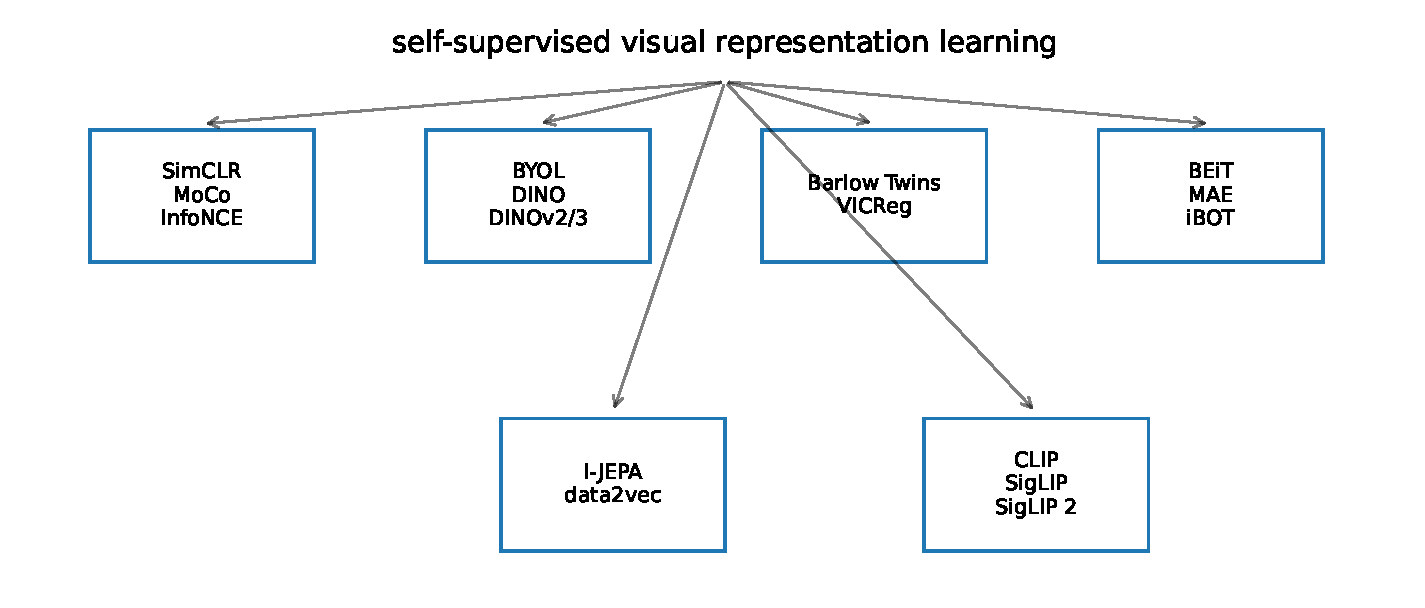
\includegraphics[width=0.97\textwidth]{fig11_10_ssl_taxonomy.pdf}
\caption{نقشه خانواده‌های اصلی یادگیری خودنظارتی بینایی. تفاوت بنیادی روش‌ها در فضای هدف، نوع ناوردایی و سازوکار جلوگیری از فروپاشی است.}
\label{fig:ssl-taxonomy}
\end{figure}

\chapter*{نقشه فشرده فصل}
\addcontentsline{toc}{chapter}{نقشه فشرده فصل}
\begin{longtable}{p{37mm}p{102mm}}
\toprule
محور & پرسش و خروجی آموزشی \\
\midrule
توکن‌سازی & وصله، توکن هم‌پوشان، توکن سلسله‌مراتبی، توکن تطبیقی و توکن وضوح بومی چه اطلاعاتی را حفظ یا حذف می‌کنند؟ \\
جبر توجه & \lr{Q}، \lr{K} و \lr{V} چگونه ساخته می‌شوند، چرا تقسیم بر $\sqrt{d_k}$ لازم است و گرادیان نرمینه چه رفتاری دارد؟ \\
مکان & مدل بدون کد مکانی چه چیزی را نمی‌داند و embedding مطلق، bias نسبی، \lr{RoPE} دوبعدی و درون‌یابی چه تفاوتی دارند؟ \\
معماری‌ها & \lr{ViT}، \lr{DeiT}، \lr{Swin}، \lr{PVT}، \lr{MViT}، \lr{MaxViT} و \lr{Hiera} چگونه مقیاس و وضوح را مدیریت می‌کنند؟ \\
کارایی & توجه پنجره‌ای، پراکنده، خطی، \lr{FlashAttention}، حذف/ادغام توکن و بسته‌بندی دنباله چه مبادله‌ای دارند؟ \\
کنتراستی & \lr{InfoNCE}، دما، batch، منفی‌ها، projection head و augmentation چگونه هندسه نمایش را تعیین می‌کنند؟ \\
خودتقطیر & \lr{BYOL}، \lr{DINO} و خانواده‌های جدید چگونه بدون منفی صریح از پاسخ ثابت اجتناب می‌کنند؟ \\
کاهش افزونگی & \lr{Barlow Twins} و \lr{VICReg} چگونه واریانس و کوواریانس را کنترل می‌کنند؟ \\
مدل‌سازی ماسک‌شده & \lr{BEiT}، \lr{MAE}، \lr{iBOT} و \lr{data2vec} در فضای هدف و معماری encoder--decoder چه تفاوتی دارند؟ \\
پیش‌بینی نهفته & \lr{I-JEPA} چرا به‌جای پیکسل، بلوک هدف را در فضای نمایش پیش‌بینی می‌کند؟ \\
مدل بنیادی & داده‌گزینی، مقیاس، ویژگی متراکم، وضوح بالا و هم‌ترازی متن در \lr{DINOv2/v3}، \lr{EVA-02} و \lr{SigLIP 2} چه نقشی دارند؟ \\
کتابخانه‌ها & \lr{PyTorch SDPA}، \lr{timm}، \lr{Transformers}، \lr{Lightly}، \lr{MMSelfSup} و مخازن رسمی چگونه در یک خط لوله قرار می‌گیرند؟ \\
ارزیابی & linear probe، \lr{kNN}، fine-tuning، بازیابی، dense transfer، عدم‌قطعیت، OOD و هزینه محاسباتی چگونه گزارش می‌شوند؟ \\
\bottomrule
\end{longtable}

\tableofcontents
\mainmatter
\setcounter{chapter}{10}
\chapter{ترنسفورمرهای بینایی و یادگیری خودنظارتی}

\begin{learningbox}
در پایان فصل، دانشجو باید بتواند:
\begin{itemize}
\item عملگر \lr{patchify/unpatchify} را با نمادگذاری تانسوری و کد پیاده‌سازی کند؛
\item تعداد توکن، پارامتر و هزینه توجه را برای وضوح و اندازه وصله دلخواه محاسبه کند؛
\item توجه مقیاس‌شده و چندسری را از روی ضرب داخلی و نرمینه استخراج کند؛
\item تفاوت embedding مکان مطلق، bias نسبی و \lr{RoPE} را تحلیل کند؛
\item یک \lr{ViT} پیش‌هنجارشده را از صفر بسازد و گرادیان آن را بررسی کند؛
\item \lr{InfoNCE} و مشتق آن نسبت به logits و دما را توضیح دهد؛
\item سازوکار ضد فروپاشی در \lr{MoCo}، \lr{BYOL}، \lr{DINO}، \lr{Barlow Twins}، \lr{VICReg}، \lr{MAE} و \lr{I-JEPA} را مقایسه کند؛
\item معیارهای تشخیص فروپاشی کامل و بعدی را محاسبه کند؛
\item یک backbone پیش‌آموخته را برای linear probe، استخراج ویژگی یا fine-tuning به‌کار گیرد؛
\item یک آزمایش خودنظارتی بازتولیدپذیر با ثبت داده، augmentation، seed، schedule، هزینه و معیار بسازد.
\end{itemize}
\end{learningbox}

\section{از پیکسل تا توکن: تغییر واحد محاسبه}
در شبکه کانولوشنی، واحد پایه محاسبه معمولاً یک مکان روی feature map است. در \lr{ViT}، تصویر ابتدا به واحدهایی تبدیل می‌شود که
در ادبیات «توکن» نام دارند. توکن لزوماً یک وصله ثابت نیست؛ می‌تواند حاصل یک کانولوشن هم‌پوشان، یک ناحیه شیء، یک خوشه از نقاط،
یک لوله زمانی در ویدئو یا یک بردار آموخته‌شده باشد. بنابراین پیش از هر بحث درباره attention باید پرسید:
\begin{quote}
\textbf{مدل دقیقاً چه چیزهایی را به‌عنوان عناصر دنباله می‌بیند و چه اطلاعاتی پیش از اولین بلوک ترنسفورمر حذف شده است؟}
\end{quote}

فرض کنید تصویر
\begin{equation}
\mat X\in\R^{H\times W\times C}
\end{equation}
با وصله مربعی $P\times P$ و بدون هم‌پوشانی تقسیم شود. اگر $P\mid H$ و $P\mid W$، تعداد وصله‌ها برابر است با
\begin{equation}
N=\frac{H}{P}\frac{W}{P}=\frac{HW}{P^2}.
\label{eq:token-count}
\end{equation}
هر وصله تخت می‌شود و با ماتریس آموختنی $\mat E\in\R^{(P^2C)\times D}$ به فضای embedding می‌رود:
\begin{equation}
\vect z_i = \operatorname{vec}(\mat X_i)\mat E+\vect b,
\qquad i=1,\ldots,N.
\label{eq:patch-proj}
\end{equation}
اگر توکن طبقه‌بندی افزوده شود، طول دنباله $N+1$ خواهد بود.

\begin{figure}[H]
\centering
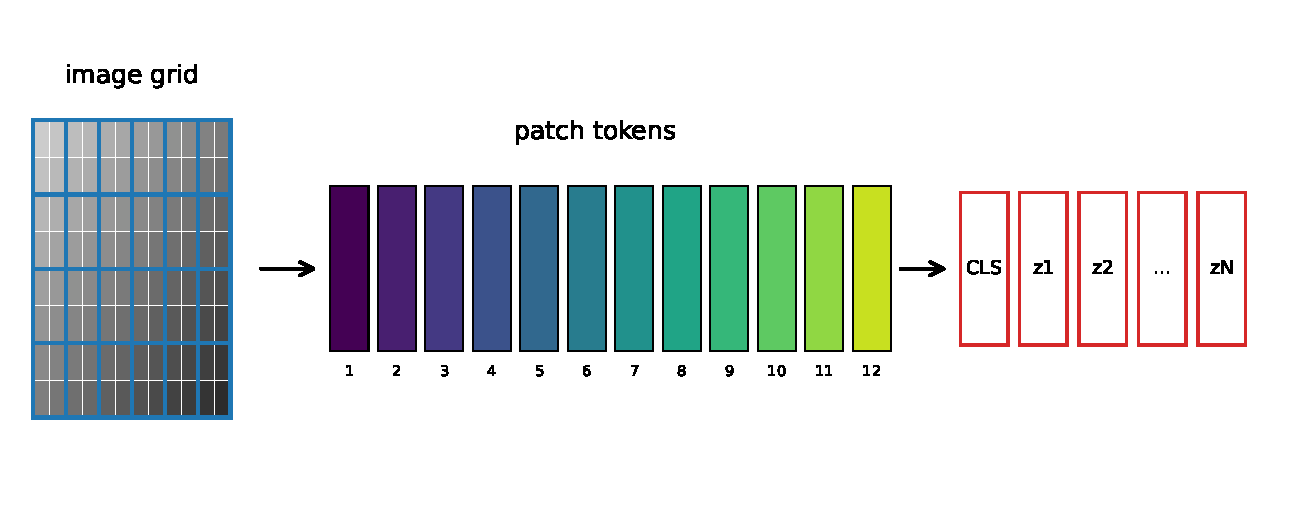
\includegraphics[width=0.96\textwidth]{fig11_01_patchify.pdf}
\caption{تبدیل شبکه پیکسلی به دنباله توکن‌ها. ترتیب خطی باید با هندسه دوبعدی و embedding مکانی سازگار باقی بماند.}
\label{fig:patchify}
\end{figure}

\subsection{وصله‌سازی یک عملگر خطی است}
عمل patchify را می‌توان با یک ماتریس جایگشتی و انتخابی نوشت. اگر تصویر برداری‌شده را $\vect x\in\R^{HWC}$ بنامیم،
آنگاه
\begin{equation}
\mat P_{\mathrm{patch}}\vect x
=\begin{bmatrix}
\operatorname{vec}(\mat X_1)\\
\vdots\\
\operatorname{vec}(\mat X_N)
\end{bmatrix}
\in\R^{N\times P^2C}.
\end{equation}
پس embedding وصله‌ها یک نگاشت خطی مرکب است:
\begin{equation}
\mat Z=(\mat P_{\mathrm{patch}}\vect x)\mat E+\mathbf{1}\vect b\trans.
\end{equation}
این مشاهده دو پیام دارد. نخست آنکه مرحله patchify ذاتاً یادگیری ندارد و تنها بازآرایی است؛ دوم آنکه projection وصله‌ها دقیقاً با یک
کانولوشن با kernel و stride برابر $P$ هم‌ارز است. در قرارداد \lr{NCHW}:
\begin{equation}
\operatorname{Conv2D}(C,D,k=P,s=P)
\quad\Longleftrightarrow\quad
\text{patchify}+\text{linear projection}.
\end{equation}
این هم‌ارزی برای انتقال وزن، export مدل و فهم تفاوت پیاده‌سازی‌ها مهم است.

\begin{workshopbox}[وصله‌سازی و بازسازی دقیق]
فایل \lr{code/patchify.py} عملگر رفت و برگشت را پیاده‌سازی می‌کند. آزمون اصلی باید خطای بازسازی صفر تولید کند؛ اگر ترتیب
محورها در \lr{permute} اشتباه باشد، تصویر ظاهراً ابعاد صحیح دارد اما پیکسل‌ها درون وصله‌ها جابه‌جا می‌شوند.
\begin{latin}
\lstinputlisting[firstline=1,lastline=42]{code/patchify.py}
\end{latin}
\end{workshopbox}

\subsection{قانون مقیاس هزینه با اندازه وصله}
هزینه attention سراسری شامل تشکیل $\mat Q\mat K\trans$ است. با حذف ثابت‌ها:
\begin{equation}
\mathcal C_{\mathrm{attn}}=\mathcal O(N^2D),
\qquad
\mathcal M_{\mathrm{attn}}=\mathcal O(N^2).
\end{equation}
با جایگذاری رابطه \eqref{eq:token-count}:
\begin{equation}
\mathcal C_{\mathrm{attn}}
=\mathcal O\!\left(\frac{H^2W^2D}{P^4}\right).
\label{eq:patch-fourth}
\end{equation}
بنابراین نصف‌کردن اندازه وصله، در وضوح ثابت، تعداد توکن را تقریباً چهار برابر و ماتریس attention را حدود شانزده برابر می‌کند.
این رابطه توضیح می‌دهد چرا تغییر ظاهراً کوچک $P=16$ به $P=8$ می‌تواند حافظه را به‌طور چشمگیر افزایش دهد.

\begin{figure}[H]
\centering
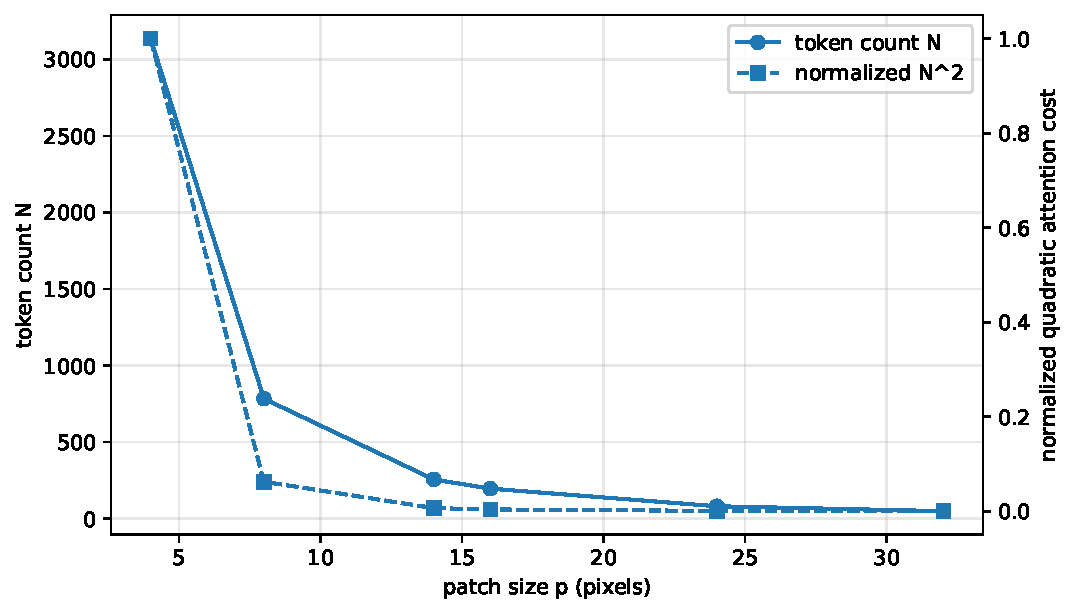
\includegraphics[width=0.74\textwidth]{fig11_02_patch_cost.pdf}
\caption{اندازه وصله نه‌تنها وضوح نمایش، بلکه هزینه درجه‌دو attention را تعیین می‌کند.}
\label{fig:patchcost}
\end{figure}

\begin{keybox}[قانون مهندسی]
در گزارش مدل، نوشتن نام \lr{ViT-B} کافی نیست. باید حداقل وضوح ورودی، اندازه وصله، تعداد توکن، batch، precision و نوع attention ذکر شود؛
زیرا یک backbone یکسان در وضوح‌های متفاوت هزینه و حتی رفتار بازنمایی متفاوتی دارد.
\end{keybox}

\subsection{اندازه وصله به‌عنوان پیشین فرکانسی}
وصله بزرگ، پیش از هر تعامل بین‌وصله‌ای، جزئیات را در یک بردار فشرده می‌کند. اگر projection اولیه نتواند مؤلفه‌های پرفرکانس را حفظ کند،
اطلاعات از دست رفته در لایه‌های بعد بازنمی‌گردد. از دید نمونه‌برداری، شبکه‌ای از توکن‌ها با گام $P$ ساخته می‌شود؛ بدون stem ضدآلیاس،
الگوهای ریز ممکن است به ساختار کاذب در شبکه توکن تبدیل شوند.

\begin{figure}[H]
\centering
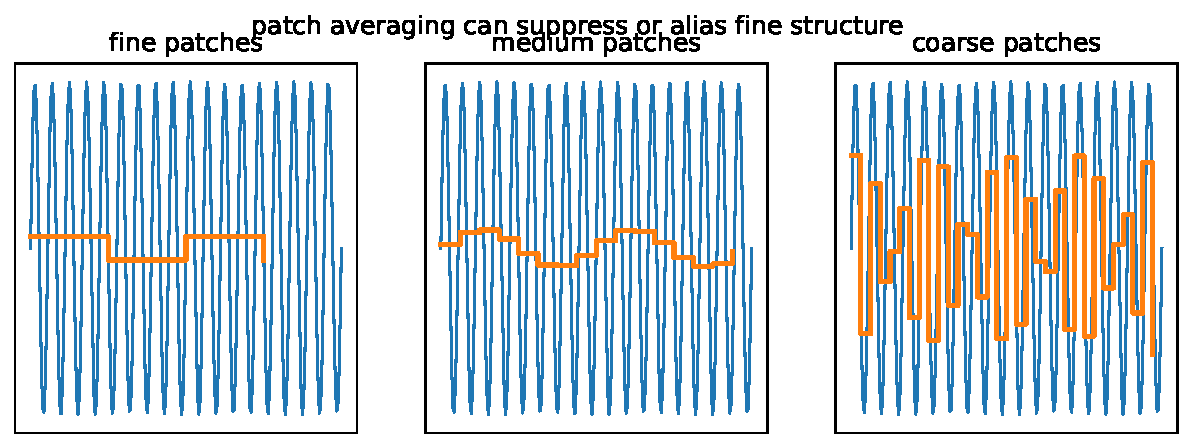
\includegraphics[width=0.9\textwidth]{fig11_03_patch_aliasing.pdf}
\caption{نمای آموزشی اثر وصله درشت بر ساختار ریز. projection آموختنی می‌تواند بهتر از میانگین ساده باشد، اما محدودیت نمونه‌برداری حذف نمی‌شود.}
\label{fig:patchalias}
\end{figure}

\subsection{توکن‌های هم‌پوشان و stem کانولوشنی}
اگر kernel بزرگ‌تر از stride باشد، وصله‌ها هم‌پوشان می‌شوند. برای kernel $K$، stride $S$ و padding $A$، تعداد توکن در هر محور
\begin{equation}
N_H=\left\lfloor\frac{H+2A-K}{S}\right\rfloor+1,
\qquad
N_W=\left\lfloor\frac{W+2A-K}{S}\right\rfloor+1.
\end{equation}
هم‌پوشانی پیوستگی مرز وصله‌ها را بهتر می‌کند، اما محاسبه و افزونگی را افزایش می‌دهد. stem چندلایه کانولوشنی می‌تواند پیش از transformer
لبه و بافت محلی را استخراج و سپس دنباله کوتاه‌تری بسازد. این طراحی در معماری‌های هیبریدی و برخی ViTهای داده‌کارآمد رایج است.

\subsection{توکن‌سازی سلسله‌مراتبی}
در backboneهای dense prediction، نگه‌داشتن وضوح ثابت در همه لایه‌ها پرهزینه است. معماری سلسله‌مراتبی پس از چند بلوک، توکن‌های مجاور را
ادغام می‌کند و تعداد کانال را افزایش می‌دهد:
\begin{equation}
(H_l,W_l,D_l)\longrightarrow
\left(\frac{H_l}{2},\frac{W_l}{2},2D_l\right).
\end{equation}
این ساختار، هرم ویژگی مشابه CNN ایجاد می‌کند و اتصال به decoderهای تشخیص و قطعه‌بندی را آسان می‌سازد.

\begin{figure}[H]
\centering
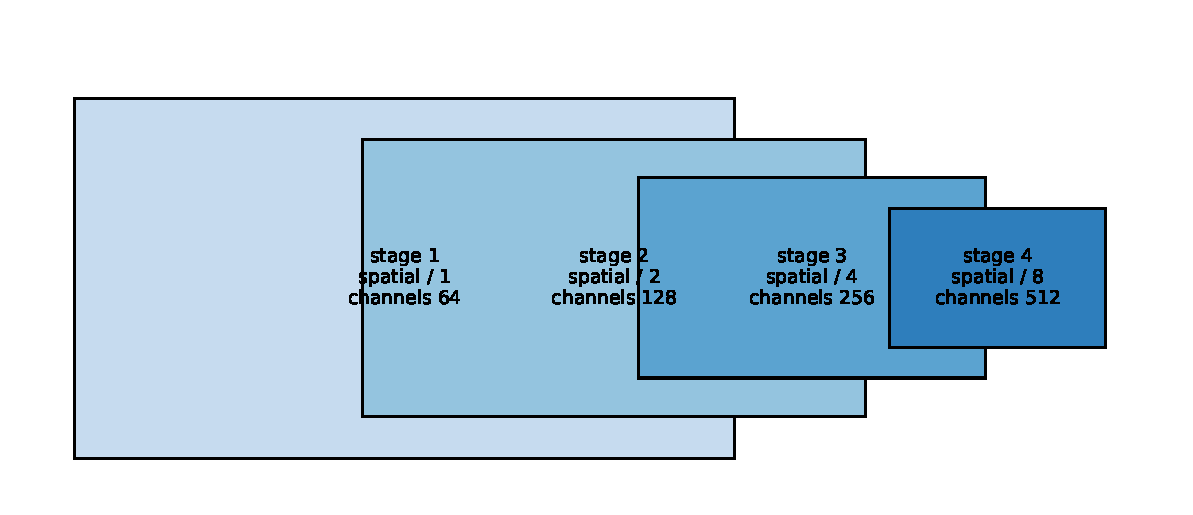
\includegraphics[width=0.9\textwidth]{fig11_08_hierarchy.pdf}
\caption{نمایش سلسله‌مراتبی با کاهش وضوح و افزایش کانال. طراحی دقیق نسبت‌ها به معماری وابسته است.}
\label{fig:hierarchy-vit}
\end{figure}

\subsection{توکن‌سازی تطبیقی: محتوا تعیین می‌کند چه چیزی دیده شود}
وصله ثابت مستقل از محتواست. در مقابل، \lr{TokenLearner} نقشه‌های توجه فضایی می‌آموزد و چند توکن خلاصه محتوامحور تولید می‌کند.
\lr{DynamicViT} در میانه شبکه، توکن‌های کم‌اهمیت را حذف می‌کند و \lr{ToMe} توکن‌های مشابه را ادغام می‌کند. اگر $N_l$ تعداد توکن در لایه $l$ باشد،
هزینه کل تقریبی
\begin{equation}
\sum_{l=1}^{L}\mathcal O(N_l^2D)
\end{equation}
است؛ بنابراین کاهش زودهنگام $N_l$ سود بیشتری دارد. با این حال، حذف توکن ممکن است ساختار کوچک یا اقلیت را نابود کند و ادغام توکن ممکن است مرزهای
اشیاء نزدیک را مخلوط سازد. معیار کارایی باید علاوه بر دقت طبقه‌بندی، وظایف متراکم و گروه‌های دشوار را نیز بررسی کند.

\begin{figure}[H]
\centering
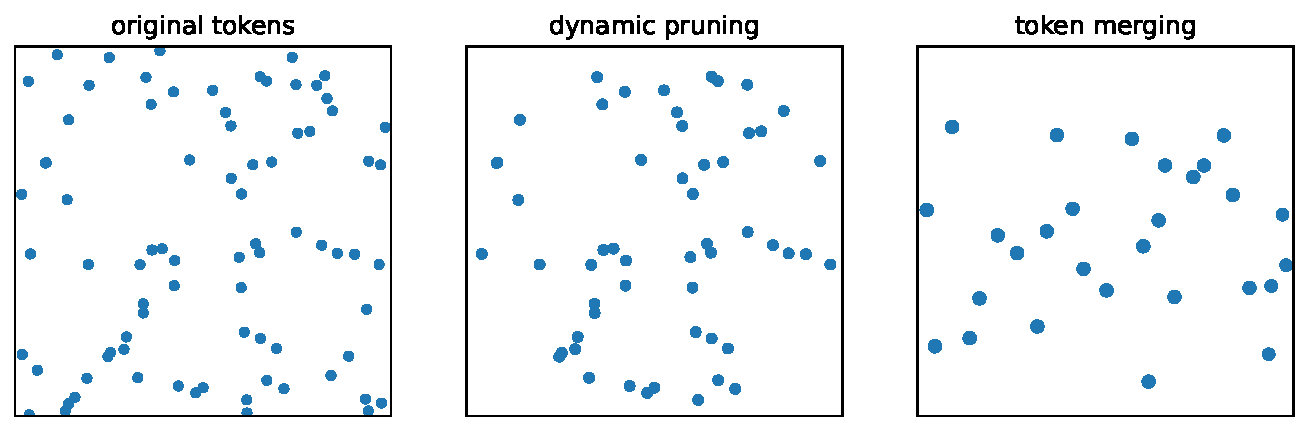
\includegraphics[width=0.94\textwidth]{fig11_20_token_efficiency.pdf}
\caption{سه راهبرد: حفظ همه توکن‌ها، حذف محتوامحور و ادغام توکن‌های مشابه. کاهش FLOPs معادل حفظ اطلاعات نیست.}
\label{fig:token-eff}
\end{figure}

\subsection{وضوح بومی و نسبت تصویر}
تغییر اندازه همه تصاویر به مربع ثابت، هندسه و مقیاس اشیاء را تغییر می‌دهد. \lr{NaViT} تصاویر با نسبت و وضوح متفاوت را به دنباله‌های با طول
متغیر تبدیل و چند دنباله را در یک بسته محاسباتی قرار می‌دهد. برای جلوگیری از توجه میان دو تصویر متفاوت، mask بلوکی لازم است:
\begin{equation}
M_{ij}=\begin{cases}
0,&s(i)=s(j),\\
-\infty,&s(i)\neq s(j),
\end{cases}
\end{equation}
که $s(i)$ شناسه تصویر مالک توکن $i$ است. \lr{FlexiViT} با تصادفی‌کردن اندازه وصله در آموزش، یک مجموعه وزن را برای چند بودجه محاسباتی آماده می‌کند.

\begin{figure}[H]
\centering
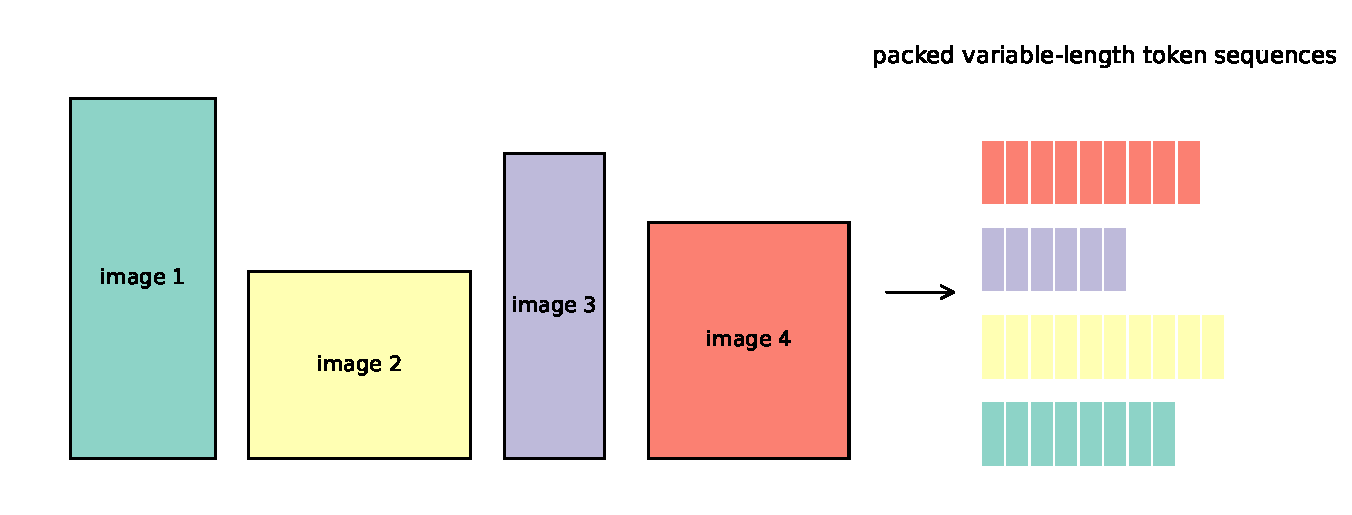
\includegraphics[width=0.93\textwidth]{fig11_19_native_pack.pdf}
\caption{بسته‌بندی دنباله‌های با طول متفاوت؛ attention mask باید مرز میان تصاویر را حفظ کند.}
\label{fig:nativepack}
\end{figure}

\begin{workshopbox}[بسته‌بندی دنباله با طول متغیر]
\begin{latin}
\lstinputlisting[firstline=1,lastline=43]{code/native_resolution_pack.py}
\end{latin}
در سامانه واقعی، استفاده از \lr{NestedTensor}، sequence packing یا kernel اختصاصی باید با profiler سنجیده شود؛ padding ساده گاهی با وجود محاسبه اضافه،
روی GPU سریع‌تر از ساختار بسیار نامنظم است.
\end{workshopbox}

\subsection{توکن شیء، ناحیه، و کد بصری گسسته}
سه مفهوم نباید با هم مخلوط شوند:
\begin{enumerate}
\item \textbf{توکن وصله:} یک مکان شبکه منظم را نمایندگی می‌کند؛
\item \textbf{توکن ناحیه/شیء:} از pooling یا query آموختنی برای یک موجودیت احتمالی ساخته می‌شود؛
\item \textbf{توکن گسسته بصری:} شاخص یک codebook مانند خروجی tokenizer در \lr{BEiT} است.
\end{enumerate}
توکن گسسته برای هدف طبقه‌بندی ماسک‌شده مناسب است، اما خطای tokenizer و ظرفیت codebook به هدف پیش‌آموزش منتقل می‌شود. توکن شیء برای شمارش و
استدلال موجودیت‌محور مفید است، اما معمولاً نیازمند سازوکار assignment یا decoder query-based است.

\subsection{توکن‌سازی در داده‌های غیر RGB}
در تصاویر چندطیفی، بعد کانال ممکن است ده‌ها یا صدها باشد. سه انتخاب رایج وجود دارد: projection مشترک همه کانال‌ها، توکن جدا برای هر کانال، یا
ترکیب توکن مکانی و embedding کانال. در حجم سه‌بعدی، وصله $P_x\times P_y\times P_z$ و در ویدئو tubelet با اندازه
$P_t\times P_h\times P_w$ است. تعداد توکن و هزینه attention اکنون با حاصل‌ضرب زمان/عمق نیز رشد می‌کند و توجه factorized یا سلسله‌مراتبی ضروری می‌شود.

\begin{warningbox}
توکن کوچک همیشه بهتر نیست. توکن کوچک، جزئیات را حفظ می‌کند اما هزینه را افزایش می‌دهد، احتمال overfitting به بافت را بالا می‌برد و ممکن است به batch کوچک‌تر
و تخمین آماری ضعیف‌تر منجر شود. اندازه وصله یک ابرپارامتر «نمایش ـ محاسبه ـ داده» است، نه صرفاً تنظیم هندسی.
\end{warningbox}

\section{جبر توجه خودکار}
\subsection{پرس‌وجو، کلید و مقدار}
برای ورودی $\mat X\in\R^{N\times D}$، سه projection خطی ساخته می‌شود:
\begin{equation}
\mat Q=\mat X\mat W_Q,\qquad
\mat K=\mat X\mat W_K,\qquad
\mat V=\mat X\mat W_V,
\end{equation}
که معمولاً $\mat Q,\mat K\in\R^{N\times d_k}$ و $\mat V\in\R^{N\times d_v}$. خروجی توجه مقیاس‌شده برابر است با
\begin{equation}
\operatorname{Attn}(\mat Q,\mat K,\mat V)
=\softmax\!\left(\frac{\mat Q\mat K\trans}{\sqrt{d_k}}+\mat M\right)\mat V.
\label{eq:sdpa}
\end{equation}
نرمینه روی بعد کلیدها اعمال می‌شود؛ در نتیجه هر سطر ماتریس وزن جمع یک دارد. $\mat M$ می‌تواند mask padding، mask علّی، پنجره‌ای یا مرز بسته‌بندی باشد.

\begin{figure}[H]
\centering
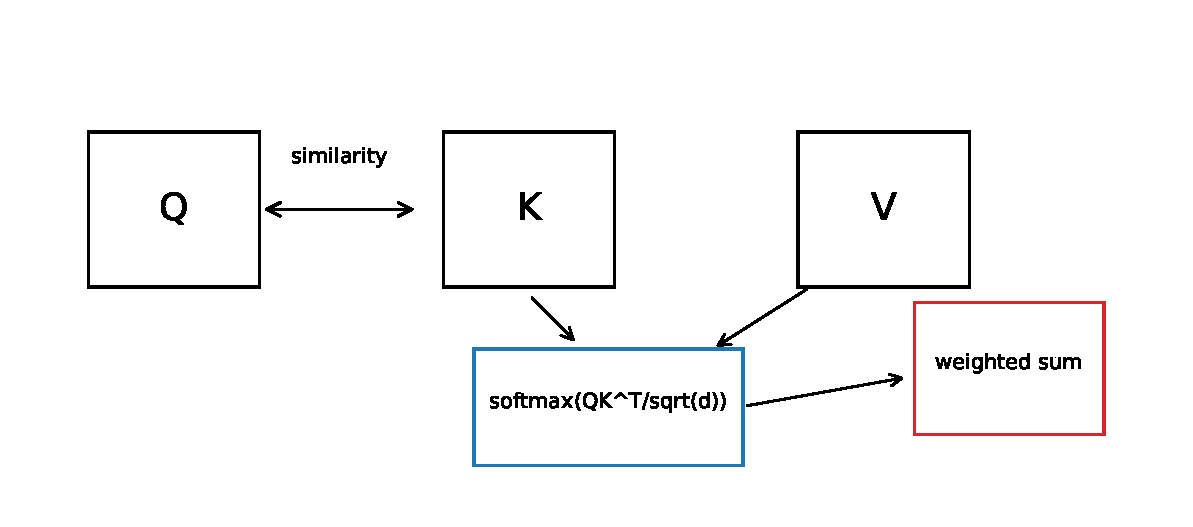
\includegraphics[width=0.91\textwidth]{fig11_04_qkv.pdf}
\caption{توجه به‌عنوان شباهت query--key و میانگین وزن‌دار value.}
\label{fig:qkv}
\end{figure}

\subsection{چرا تقسیم بر $\sqrt{d_k}$؟}
فرض کنید مؤلفه‌های query و key مستقل، با میانگین صفر و واریانس یک باشند. برای logit
\begin{equation}
s_{ij}=\vect q_i\trans\vect k_j=\sum_{r=1}^{d_k}q_{ir}k_{jr},
\end{equation}
داریم
\begin{equation}
\E[s_{ij}]=0,
\qquad
\Var(s_{ij})=d_k.
\end{equation}
با رشد $d_k$، logits بزرگ و softmax اشباع می‌شود. مقیاس $1/\sqrt{d_k}$ واریانس را تقریباً یک نگه می‌دارد و گرادیان را در ناحیه قابل استفاده حفظ می‌کند.
این استدلال دقیقاً اثبات بهینگی نیست؛ وابستگی مؤلفه‌ها، normalization و وزن‌های آموخته‌شده فرض استقلال را نقض می‌کنند، اما مقیاس از رشد سیستماتیک جلوگیری می‌کند.

\subsection{توجه به‌عنوان رگرسیون هسته‌ای وابسته به داده}
برای query ثابت $i$، وزن
\begin{equation}
a_{ij}=\frac{\exp(\vect q_i\trans\vect k_j/\sqrt{d_k})}
{\sum_m\exp(\vect q_i\trans\vect k_m/\sqrt{d_k})}
\end{equation}
یک kernel نرمال‌شده است و خروجی
\begin{equation}
\vect y_i=\sum_j a_{ij}\vect v_j
\end{equation}
مشابه رگرسیون Nadaraya--Watson در فضای ویژگی است، با این تفاوت که metric و مقادیر هم‌زمان آموخته می‌شوند. همچنین می‌توان attention را پیام‌رسانی روی یک گراف کامل داده‌محور دانست که وزن یال‌ها در هر نمونه تغییر می‌کند.

\subsection{گرادیان نرمینه}
برای $\vect a=\softmax(\vect s)$، ژاکوبین
\begin{equation}
\frac{\partial a_i}{\partial s_j}
=a_i(\delta_{ij}-a_j)
\end{equation}
یا به شکل ماتریسی
\begin{equation}
\mat J_{\mathrm{softmax}}=\diag(\vect a)-\vect a\vect a\trans
\end{equation}
است. اگر توزیع بسیار تیز شود، بیشتر $a_i$ها نزدیک صفر و یک مقدار نزدیک یک می‌شود؛ در این حالت بسیاری از عناصر ژاکوبین کوچک‌اند. از این رو دما، مقیاس logits و normalization نه‌فقط خروجی بلکه شرطی‌بودن بهینه‌سازی را تغییر می‌دهند.

\subsection{توجه چندسری}
در توجه چندسری، فضای embedding به $h$ زیرفضا تقسیم می‌شود:
\begin{equation}
\operatorname{MHA}(\mat X)
=\operatorname{Concat}(\mat O_1,\ldots,\mat O_h)\mat W_O,
\end{equation}
\begin{equation}
\mat O_r=\operatorname{Attn}(\mat X\mat W_Q^{(r)},\mat X\mat W_K^{(r)},\mat X\mat W_V^{(r)}).
\end{equation}
سرها می‌توانند روابط مکانی یا معنایی متفاوتی بیاموزند، اما هیچ تضمینی برای تخصص‌یافتگی یا عدم افزونگی وجود ندارد. pruning سرها و تحلیل شباهت نشان می‌دهد
بعضی سرها قابل حذف‌اند؛ بنابراین «تعداد سر بیشتر» ظرفیت مؤثر را لزوماً به همان نسبت افزایش نمی‌دهد.

\begin{figure}[H]
\centering
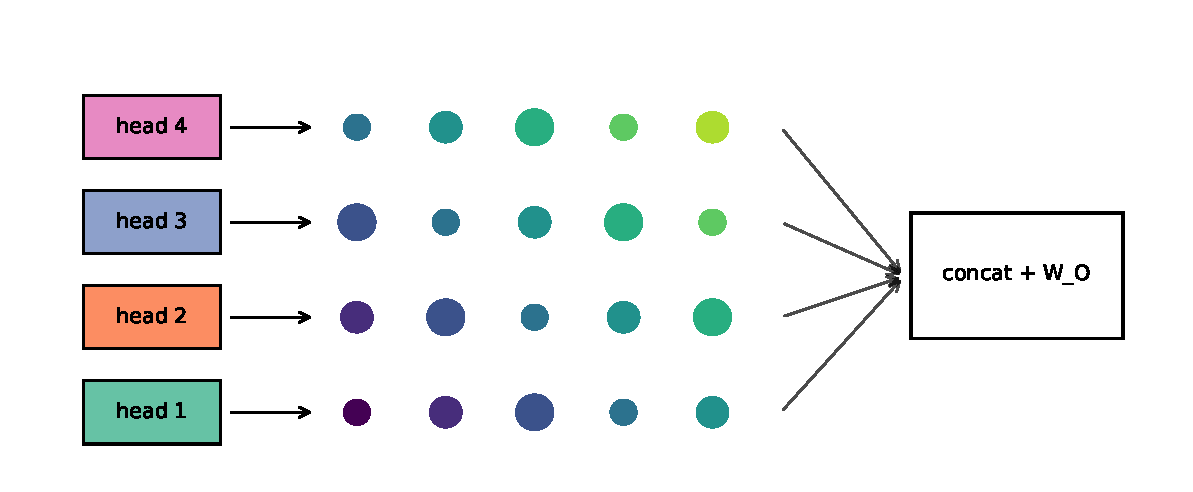
\includegraphics[width=0.9\textwidth]{fig11_05_multihead.pdf}
\caption{هر سر projection و ماتریس وزن مستقل دارد؛ خروجی‌ها الحاق و دوباره projection می‌شوند.}
\label{fig:multihead}
\end{figure}

\subsection{بلوک ترنسفورمر پیش‌هنجارشده}
یک بلوک رایج \lr{Pre-LN} به صورت
\begin{align}
\mat U_l &= \mat X_l+\operatorname{DropPath}\!\left(\operatorname{MHA}(\LN(\mat X_l))\right),\\
\mat X_{l+1} &= \mat U_l+\operatorname{DropPath}\!\left(\operatorname{MLP}(\LN(\mat U_l))\right)
\end{align}
است. مسیر هویت باعث می‌شود گرادیان یک مسیر مستقیم داشته باشد. در \lr{Post-LN}، normalization پس از جمع residual می‌آید. Pre-LN معمولاً برای شبکه‌های عمیق پایدارتر است، هرچند recipeهای جدید با scaling و initialization می‌توانند Post-LN را نیز قابل آموزش سازند.

MLP معمولاً
\begin{equation}
\operatorname{MLP}(\vect x)=\mat W_2\,\phi(\mat W_1\vect x+\vect b_1)+\vect b_2
\end{equation}
با نسبت گسترش $r=D_{\mathrm{hidden}}/D$ است. نسخه‌های gated مانند \lr{SwiGLU} دو projection می‌سازند و حاصل‌ضرب دروازه‌ای را به‌کار می‌برند.

\begin{workshopbox}[ساخت ViT آموزشی با kernel بهینه توجه]
\begin{latin}
\lstinputlisting[firstline=1,lastline=103]{code/minimal_vit.py}
\end{latin}
این کد از \lr{torch.nn.functional.scaled\_dot\_product\_attention} استفاده می‌کند. روی سخت‌افزار پشتیبانی‌شده، PyTorch می‌تواند backend بهینه را انتخاب کند؛ با این حال mask، dtype، dropout و شکل تانسور تعیین می‌کنند fast path فعال شود یا نه.
\end{workshopbox}

\subsection{آیا نقشه attention توضیح مدل است؟}
ماتریس attention نشان می‌دهد valueها چگونه در یک لایه مخلوط شده‌اند، اما به‌تنهایی اثر نهایی یک ورودی بر تصمیم را نشان نمی‌دهد. residual، MLP، چند لایه و projection خروجی مسیرهای دیگری می‌سازند. برای تفسیر باید attention rollout، gradient-weighted attention، perturbation و آزمون علی مقایسه شوند. نقشه زیبا بدون آزمون حساسیت می‌تواند گمراه‌کننده باشد.

\section{اطلاعات مکانی: مدل باید بداند توکن کجاست}
بدون embedding مکانی، self-attention نسبت به جایگشت توکن‌ها هم‌ورداست. اگر $\mat \Pi$ ماتریس جایگشت باشد:
\begin{equation}
\operatorname{Attn}(\mat\Pi\mat X)
=\mat\Pi\operatorname{Attn}(\mat X)
\end{equation}
در نتیجه مدل ترتیب شبکه تصویر را از محتوای توکن‌ها به‌تنهایی نمی‌داند. اطلاعات مکان باید به‌صورت مطلق، نسبی یا ضمنی افزوده شود.

\subsection{embedding مطلق آموختنی}
در ViT اولیه، ماتریس $\mat P\in\R^{(N+1)\times D}$ به توکن‌ها افزوده می‌شود:
\begin{equation}
\mat Z_0=[\vect z_{\mathrm{cls}};\mat Z_{\mathrm{patch}}]+\mat P.
\end{equation}
مزیت آن سادگی است. ضعف آن وابستگی به grid آموزش است. برای وضوح جدید، بخش دوبعدی embedding به شبکه تبدیل و با interpolation تغییر اندازه می‌یابد. interpolation یک فرض smoothness تحمیل می‌کند و برای تغییر شدید نسبت تصویر یا patch size ممکن است artefact بسازد.

\subsection{کد سینوسی دوبعدی}
می‌توان موقعیت سطر و ستون را جداگانه با سینوس/کسینوس کد کرد. برای بعد زوج:
\begin{align}
PE_{(p,2i)}&=\sin(p/10000^{2i/D}),\\
PE_{(p,2i+1)}&=\cos(p/10000^{2i/D}).
\end{align}
در دوبعد، بخشی از کانال‌ها به $x$ و بخشی به $y$ اختصاص می‌یابد. این کد پارامتر ندارد و extrapolation طول را ممکن می‌کند، اما هندسه فرکانسی آن لزوماً برای همه داده‌ها بهینه نیست.

\subsection{bias مکانی نسبی}
به‌جای افزودن بردار به توکن، bias وابسته به جابه‌جایی به logit attention افزوده می‌شود:
\begin{equation}
s_{ij}=\frac{\vect q_i\trans\vect k_j}{\sqrt{d_k}}+b_{\Delta x_{ij},\Delta y_{ij}}.
\end{equation}
در پنجره ثابت، جدول bias کوچک است. برای اندازه‌های متغیر می‌توان تابع پیوسته یا تجزیه محوری ساخت. bias نسبی برای انتقال مکانی طبیعی‌تر است، اما مرزها و clipping جابه‌جایی باید دقیق تعریف شوند.

\subsection{RoPE دوبعدی}
\lr{RoPE} هر جفت مؤلفه query/key را با زاویه وابسته به موقعیت می‌چرخاند. در یک بعد:
\begin{equation}
\vect q_p'=\mat R(p)\vect q_p,
\qquad
\vect k_q'=\mat R(q)\vect k_q,
\end{equation}
و ضرب داخلی به اختلاف $q-p$ وابسته می‌شود:
\begin{equation}
(\mat R(p)\vect q)\trans(\mat R(q)\vect k)
=\vect q\trans\mat R(q-p)\vect k.
\end{equation}
در تصویر، ابعاد به چرخش‌های مربوط به محور افقی و عمودی تقسیم می‌شوند. انتخاب فرکانس و scaling برای تغییر وضوح مهم است.

\begin{figure}[H]
\centering
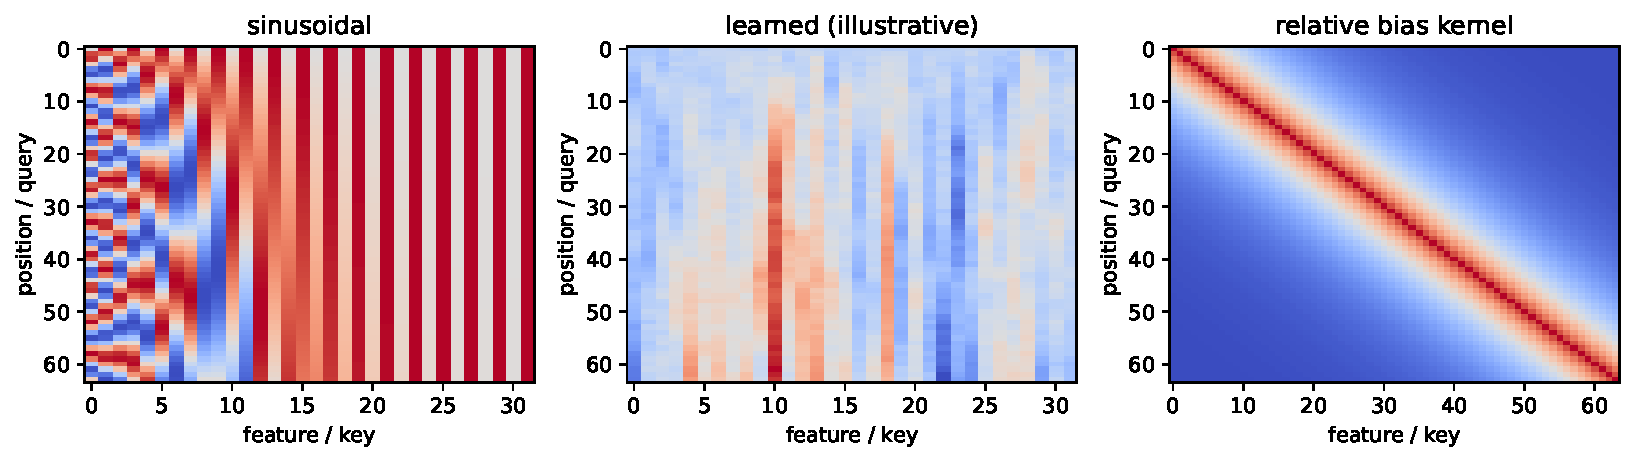
\includegraphics[width=0.96\textwidth]{fig11_06_position.pdf}
\caption{سه نمایش آموزشی از اطلاعات مکان: کد سینوسی، embedding آموختنی و kernel نسبی.}
\label{fig:position}
\end{figure}

\begin{warningbox}
کدگذاری مکان می‌تواند «سوگیری مکان» بسازد: مدل ممکن است اشیاء را بر اساس جای معمول در داده تشخیص دهد. آزمون انتقال، crop غیرمرکزی، tile shuffle و داده‌های بدون جهت ترجیحی برای ممیزی این مسئله ضروری‌اند.
\end{warningbox}

\section{Vision Transformer از ابتدا تا یک backbone عمومی}
\subsection{معماری پایه ViT}
یک ViT طبقه‌بندی معمولاً شامل مراحل زیر است:
\begin{enumerate}
\item تبدیل تصویر به $N$ توکن وصله و projection به بعد $D$؛
\item افزودن توکن \lr{CLS} و embedding مکان؛
\item عبور از $L$ بلوک transformer؛
\item استفاده از توکن \lr{CLS} یا میانگین توکن‌ها؛
\item یک سر خطی برای وظیفه پایین‌دست.
\end{enumerate}
اگر نسبت MLP برابر $r$ و تعداد سرها $h$ باشد، تعداد پارامتر تقریبی هر بلوک، با صرف‌نظر از bias و normalization،
\begin{equation}
4D^2+2rD^2=(4+2r)D^2
\end{equation}
است؛ بخش $4D^2$ از QKV و projection خروجی و بخش $2rD^2$ از دو لایه MLP می‌آید. بنابراین برخلاف تصور رایج، در بسیاری از ViTها MLP سهمی هم‌اندازه یا بزرگ‌تر از attention در پارامتر و محاسبه دارد.

هزینه تقریبی یک بلوک:
\begin{equation}
\mathcal C\approx 4ND^2+2N^2D+2rND^2.
\label{eq:vit-cost}
\end{equation}
برای $N$ کوچک، projectionها و MLP غالب‌اند؛ برای وضوح بالا، جمله $N^2D$ غالب می‌شود. این تفکیک توضیح می‌دهد چرا کاهش توکن در مدل بزرگ همیشه همان سودی را ندارد که محاسبه فقط از روی $N^2$ وعده می‌دهد.

\subsection{توکن CLS یا pooling؟}
توکن CLS یک query آموختنی است که باید اطلاعات لازم برای تصمیم را جمع‌آوری کند. میانگین‌گیری توکن‌ها، فرض می‌کند همه مکان‌ها سهمی متناسب دارند. انتخاب میان این دو به recipe و پیش‌آموزش وابسته است. در مدل‌های خودنظارتی، گاهی توکن CLS برای ویژگی جهانی و patch tokenها برای انتقال متراکم به‌کار می‌روند. گزارش فقط «خروجی backbone» کافی نیست؛ باید مشخص شود کدام لایه و کدام pooling استفاده شده است.

\subsection{ViT و نیاز به داده}
ViT اولیه با پیش‌آموزش بزرگ‌مقیاس درخشید، زیرا locality سخت CNN را ندارد و باید بخشی از ساختار را از داده بیاموزد. اما نتیجه «ترنسفورمر همیشه به صدها میلیون تصویر نیاز دارد» نادرست است. recipeهای قوی augmentation، regularization، distillation و self-supervised pretraining می‌توانند مدل را روی داده متوسط آموزش دهند. تفاوت اصلی، مقدار پیشین معماری و محل ورود آن است.

\subsection{DeiT: داده‌کارآمدی و توکن تقطیر}
\lr{DeiT} با recipe آموزشی دقیق و distillation، ViT را روی ImageNet بدون پیش‌آموزش خارجی رقابتی کرد. توکن تقطیر $\vect z_{\mathrm{dist}}$ در کنار CLS وارد دنباله می‌شود و یک سر جدا خروجی معلم را تقلید می‌کند. تابع هدف نمونه:
\begin{equation}
\mathcal L=\lambda\,\CE(y,p_{\mathrm{cls}})+(1-\lambda)\,\CE(\widehat y_T,p_{\mathrm{dist}}).
\end{equation}
این طراحی نشان می‌دهد token می‌تواند نقش یک رابط وظیفه‌ای داشته باشد، نه فقط نماینده یک وصله.

\subsection{هیبرید CNN--Transformer}
CNN stem یا backbone اولیه، feature map محلی می‌سازد و transformer روابط دوربرد را مدل می‌کند. این طراحی در داده کم یا وظایف با بافت محلی قوی مفید است، اما تفسیر هزینه و resolution پیچیده‌تر می‌شود. مقایسه منصفانه باید recipe، تعداد پارامتر، FLOPs و latency یکسان را در نظر گیرد؛ نام «هیبرید» به‌تنهایی مزیت نیست.

\section{معماری‌های سلسله‌مراتبی و attention محلی}
\subsection{Pyramid Vision Transformer}
\lr{PVT} نمایش چندمقیاسی می‌سازد و تعداد توکن را در stageها کاهش می‌دهد. spatial-reduction attention کلید و value را روی شبکه کم‌وضوح‌تر محاسبه می‌کند؛ اگر نسبت کاهش $R$ باشد، تعداد key/value تقریباً $N/R^2$ است و هزینه query-key به
\begin{equation}
\mathcal O\!\left(\frac{N^2D}{R^2}\right)
\end{equation}
کاهش می‌یابد. کاهش شدید ممکن است جزئیات کوچک را در key/value حذف کند.

\subsection{Swin و پنجره جابه‌جا‌شونده}
در \lr{Swin}، attention داخل پنجره $M\times M$ انجام می‌شود. اگر تعداد کل توکن $N$ باشد، هزینه تقریبی
\begin{equation}
\mathcal O(NM^2D)
\end{equation}
است؛ نسبت به $N$ خطی است وقتی $M$ ثابت باشد. اگر پنجره‌ها در همه لایه‌ها ثابت بمانند، تبادل اطلاعات میان پنجره‌ها محدود می‌شود. جابه‌جایی پنجره در بلوک بعدی، توکن‌هایی را که قبلاً در پنجره‌های جدا بودند کنار هم می‌آورد.

\begin{figure}[H]
\centering
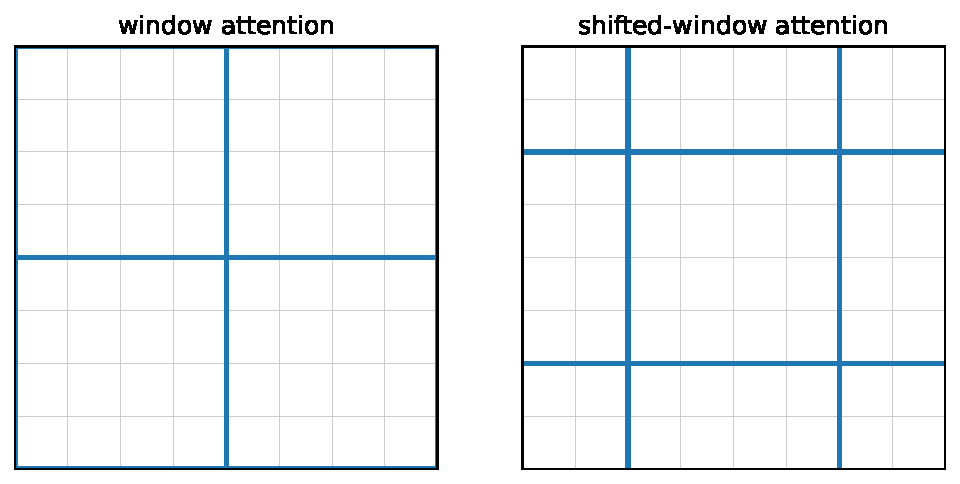
\includegraphics[width=0.82\textwidth]{fig11_07_windows.pdf}
\caption{attention پنجره‌ای و جابه‌جایی پنجره برای ارتباط بین نواحی. در پیاده‌سازی واقعی، cyclic shift و mask مرزی استفاده می‌شود.}
\label{fig:swin}
\end{figure}

\subsection{MViT، pooling attention و Hiera}
\lr{MViT} اندازه دنباله و بعد کانال را در طول شبکه تغییر می‌دهد و pooling را داخل سازوکار attention وارد می‌کند. \lr{Hiera} نشان می‌دهد با پیش‌آموزش ماسک‌شده قوی، می‌توان بخش‌هایی از پیچیدگی معماری سلسله‌مراتبی را حذف و backbone ساده‌تر و سریع‌تری ساخت. پیام آموزشی مهم این است:
\begin{quote}
قدرت نهایی حاصل برهم‌کنش معماری و objective پیش‌آموزش است؛ نمی‌توان backbone را مستقل از روش آموزش رتبه‌بندی کرد.
\end{quote}

\subsection{MaxViT و attention چندمحوری}
\lr{MaxViT} attention محلی بلوکی را با attention شبکه‌ای یا dilated ترکیب می‌کند تا در هر بلوک هم تعامل محلی و هم مسیرهای دوربرد داشته باشد. اگر تنها پنجره محلی باشد، قطر گراف ارتباطی با عمق کاهش می‌یابد؛ محور دوم ارتباط سراسری را با هزینه خطی‌تر فراهم می‌کند.

\subsection{میدان تعامل و فاصله attention}
در CNN میدان پذیرش با kernel و stride تعیین می‌شود. در attention سراسری، از اولین لایه همه توکن‌ها بالقوه مرتبط‌اند، اما وزن واقعی می‌تواند محلی باشد. فاصله میانگین attention برای سر $h$ و لایه $l$ را می‌توان نوشت:
\begin{equation}
D_{l,h}=\frac{1}{N}\sum_i\sum_j a^{(l,h)}_{ij}\,\norm{\vect p_i-\vect p_j}_2.
\end{equation}
این معیار ظرفیت نظری را با استفاده واقعی مقایسه می‌کند، ولی بدون تحلیل value و gradient کامل نیست.

\begin{figure}[H]
\centering
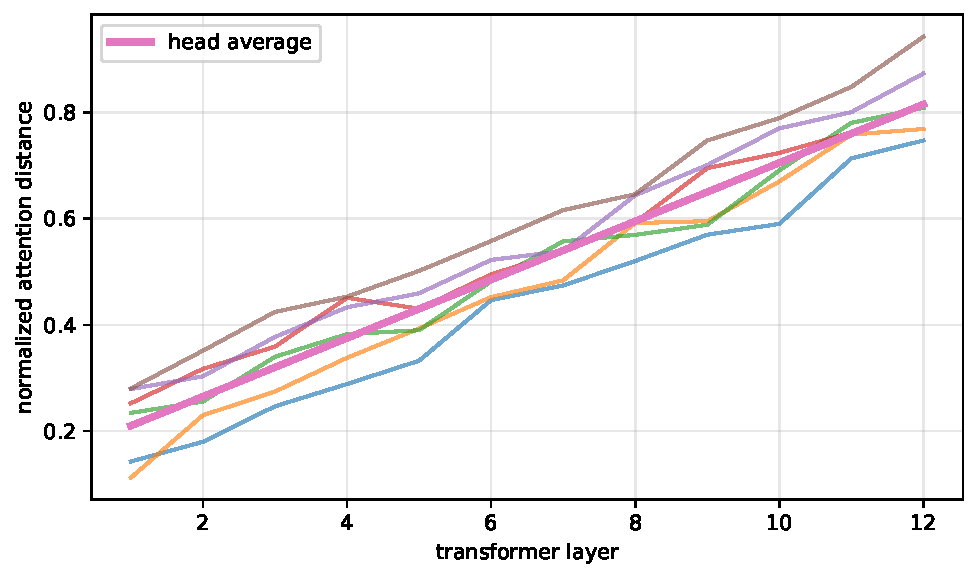
\includegraphics[width=0.76\textwidth]{fig11_21_attention_distance.pdf}
\caption{نمونه آموزشی رشد فاصله attention با عمق؛ سرها می‌توانند رفتارهای متفاوتی داشته باشند.}
\label{fig:attndistance}
\end{figure}

\section{کارایی attention: FLOPs، حافظه و حرکت داده}
\subsection{مسئله درجه‌دو}
ماتریس logits برای $B$ batch، $h$ سر و $N$ توکن دارای $BhN^2$ عنصر است. در precision شانزده‌بیتی، فقط نگه‌داری یک tensor با $B=32$، $h=12$ و $N=1024$ حدود
\begin{equation}
32\times12\times1024^2\times2\ \text{bytes}
\approx 768\ \text{MiB}
\end{equation}
نیاز دارد؛ بدون gradient و tensorهای میانی. بنابراین مسئله attention فقط تعداد ضرب نیست، بلکه جابه‌جایی داده و materialization ماتریس است.

\begin{figure}[H]
\centering
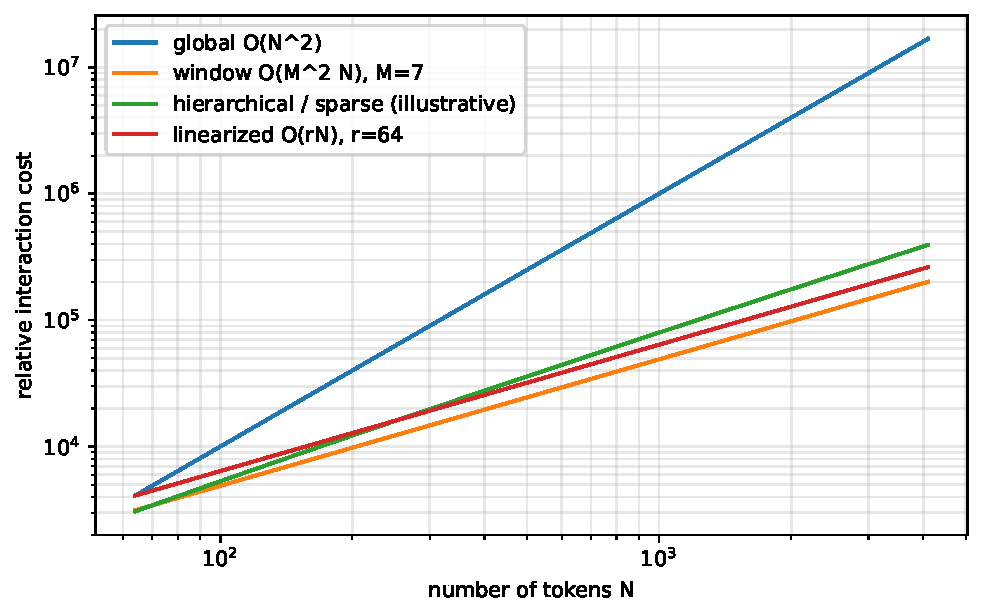
\includegraphics[width=0.78\textwidth]{fig11_09_complexity.pdf}
\caption{رشد هزینه تعامل برای چند خانواده attention. منحنی‌ها مقیاس مفهومی‌اند و ثابت‌های kernel و سخت‌افزار را نشان نمی‌دهند.}
\label{fig:attncomplexity}
\end{figure}

\subsection{خانواده‌های کاهش هزینه}
\begin{enumerate}
\item \textbf{محلی/پنجره‌ای:} هر query فقط زیرمجموعه‌ای از همسایه‌ها را می‌بیند؛
\item \textbf{پراکنده ساختاری:} الگوی اتصال block، محوری، dilated یا global-token است؛
\item \textbf{کاهش key/value:} query کامل با key/value کم‌وضوح تعامل می‌کند؛
\item \textbf{کم‌رتبه یا kernelized:} softmax attention با فاکتوربندی یا feature map تقریب زده می‌شود؛
\item \textbf{کاهش توکن:} pruning، merging یا TokenLearner طول دنباله را کم می‌کند؛
\item \textbf{الگوریتم دقیق حافظه‌کارآمد:} خروجی exact با tiling و recomputation محاسبه می‌شود.
\end{enumerate}
هیچ روش واحدی برای همه اندازه‌ها و سخت‌افزارها برتر نیست. attention خطی ممکن است FLOPs کمتری داشته باشد، اما kernel نامناسب یا ثابت بزرگ، latency را بدتر کند.

\subsection{FlashAttention: تغییر الگوریتم، نه تقریب تابع}
\lr{FlashAttention} attention دقیق را با tiling محاسبه می‌کند تا خواندن/نوشتن حافظه پرهزینه کاهش یابد و ماتریس کامل $N\times N$ در حافظه اصلی materialize نشود. softmax به‌صورت بلوکی و پایدار با نگه‌داری ماکزیمم و مجموع نرمال‌ساز به‌روزرسانی می‌شود. برای دو بلوک logits، اگر $m_1,m_2$ ماکزیمم‌های محلی باشند، ماکزیمم ترکیبی
\begin{equation}
m=\max(m_1,m_2)
\end{equation}
و مجموع نمایی ترکیبی با rescale:
\begin{equation}
\ell=e^{m_1-m}\ell_1+e^{m_2-m}\ell_2
\end{equation}
محاسبه می‌شود. این هویت اجازه می‌دهد softmax streaming باشد.

\begin{librarybox}[PyTorch SDPA]
تابع \lr{scaled\_dot\_product\_attention} یک رابط سطح بالا برای attention مقیاس‌شده است و بسته به device، dtype، شکل و mask می‌تواند backend متفاوتی انتخاب کند. برای benchmark باید warm-up، synchronization، forward/backward، dropout و طول دنباله واقعی ثبت شود. \lr{nn.MultiheadAttention} در شرایط مناسب از همین kernelهای بهینه استفاده می‌کند.
\end{librarybox}

\begin{workshopbox}[benchmark کوچک attention]
\begin{latin}
\lstinputlisting{code/benchmark_attention.py}
\end{latin}
خروجی CPU این بسته فقط smoke test است. هیچ عدد آن نباید به‌عنوان benchmark عمومی گزارش شود. روی GPU باید \lr{torch.cuda.synchronize()} و اندازه‌گیری peak memory افزوده شود.
\end{workshopbox}

\subsection{کاهش توکن و خطر سوگیری}
اگر score توکن $g_i$ باشد، pruning سخت توکن‌های $g_i<\tau$ را حذف می‌کند. در آموزش، تصمیم گسسته با mask نرم، Gumbel، straight-through یا loss بودجه تقریب زده می‌شود. یک تابع نمونه:
\begin{equation}
\mathcal L=\mathcal L_{\mathrm{task}}+\lambda\left(\frac{1}{N}\sum_i m_i-\rho\right)^2.
\end{equation}
توکن‌های مربوط به شیء کوچک ممکن است score پایین اما اهمیت بالا داشته باشند. برای کاربرد پزشکی یا صنعتی، ارزیابی باید بر حسب اندازه ضایعه/شیء و ناحیه‌های کم‌نمونه تفکیک شود.

\section{یادگیری خودنظارتی: مسئله دقیق چیست؟}
داده بدون برچسب $\{\vect x_i\}_{i=1}^n$ داریم و می‌خواهیم encoder
\begin{equation}
\vect h=f_\theta(\vect x)
\end{equation}
نمایشی بسازد که با هزینه برچسب کم به وظایف گوناگون منتقل شود. خودنظارتی از تبدیل‌ها، ماسک، زمان، چندوجهی‌بودن یا ساختار نمونه، هدف مصنوعی می‌سازد. کیفیت هدف با سه پرسش سنجیده می‌شود:
\begin{enumerate}
\item کدام اطلاعات باید \textbf{ناوردا} شوند؟
\item کدام اطلاعات باید \textbf{حفظ} شوند؟
\item چه چیزی مانع پاسخ ثابت یا نمایش کم‌رتبه می‌شود؟
\end{enumerate}

\subsection{دو نما و گروه تبدیل}
اگر $t_1,t_2\sim\mathcal T$ دو augmentation باشند، نماها
\begin{equation}
\widetilde{\vect x}^{(1)}=t_1(\vect x),\qquad
\widetilde{\vect x}^{(2)}=t_2(\vect x)
\end{equation}
باید هویت معنایی مشترک داشته باشند. انتخاب $\mathcal T$ در واقع تعریف عملی «چه چیزی یکسان است» است. crop شدید برای طبقه‌بندی شیء مفید است، اما در پزشکی ممکن است cropها دو ناحیه با تشخیص متفاوت بسازند. تغییر رنگ برای اشیاء طبیعی می‌تواند مطلوب باشد، اما در پاتولوژی یا سنجش‌ازدور اطلاعات تشخیصی را حذف کند.

\begin{figure}[H]
\centering
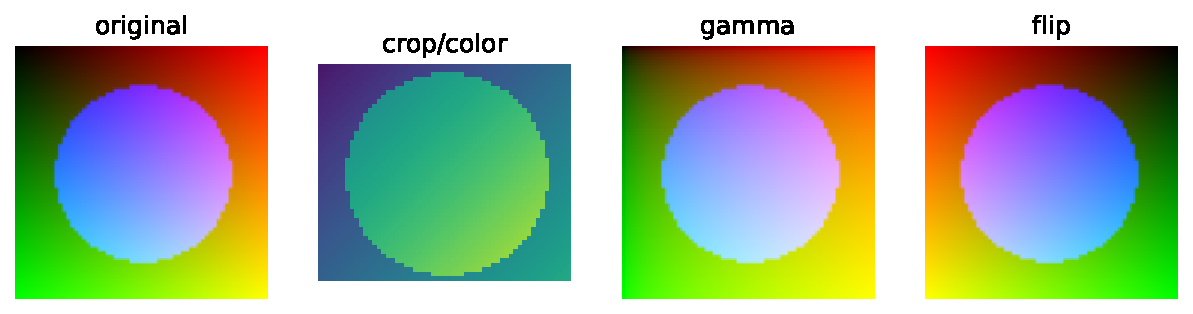
\includegraphics[width=0.9\textwidth]{fig11_13_augmentations.pdf}
\caption{augmentation سیگنال نظارت را تعریف می‌کند. ترکیب نامناسب می‌تواند positive pair غلط بسازد.}
\label{fig:augment}
\end{figure}

\begin{principlebox}
در یادگیری خودنظارتی، augmentation یک مرحله تزئینی preprocessing نیست؛ بخشی از مدل آماری و تابع هدف است. هر مقاله باید rationale دامنه‌ای برای هر تبدیل ارائه کند.
\end{principlebox}

\subsection{سه فضای متفاوت}
معمولاً encoder نمایش $\vect h$، projection head بردار $\vect z=g(\vect h)$ و سر پایین‌دست خروجی $\vect y$ را می‌سازند. loss خودنظارتی اغلب روی $\vect z$ اعمال می‌شود، اما انتقال از $\vect h$ انجام می‌شود. projection head می‌تواند اطلاعات لازم برای ناوردایی pretext را از فضای عمومی‌تر $\vect h$ جدا کند. حذف این تفکیک گاهی performance انتقال را کاهش می‌دهد.

\section{یادگیری کنتراستی و InfoNCE}
\subsection{تابع هدف NT-Xent}
برای batch شامل $B$ تصویر و دو نمای هر تصویر، $2B$ embedding نرمال‌شده داریم. اگر $i$ و $j$ یک زوج مثبت باشند، loss جهت‌دار
\begin{equation}
\ell_{i\rightarrow j}
=-\log
\frac{\exp(\operatorname{sim}(\vect z_i,\vect z_j)/\tau)}
{\sum_{k\neq i}\exp(\operatorname{sim}(\vect z_i,\vect z_k)/\tau)}
\label{eq:infonce}
\end{equation}
است، که معمولاً
\begin{equation}
\operatorname{sim}(\vect a,\vect b)=\frac{\vect a\trans\vect b}{\norm{\vect a}_2\norm{\vect b}_2}
\end{equation}
و $\tau>0$ دماست. loss نهایی میانگین دو جهت و همه positiveهاست.

اگر logitها را $u_{ik}=\operatorname{sim}(\vect z_i,\vect z_k)/\tau$ و احتمال softmax را $p_{ik}$ بنامیم:
\begin{equation}
\frac{\partial\ell_i}{\partial u_{ik}}=p_{ik}-\mathbb 1[k=j].
\end{equation}
از آنجا که $u=s/\tau$:
\begin{equation}
\frac{\partial\ell_i}{\partial s_{ik}}
=\frac{1}{\tau}\left(p_{ik}-\mathbb 1[k=j]\right).
\label{eq:temp-grad}
\end{equation}
پس دمای کوچک هم توزیع را تیز و هم اندازه گرادیان را بزرگ می‌کند. دمای بسیار کم می‌تواند روی negativeهای سخت یا حتی false negativeها تمرکز افراطی ایجاد کند.

\begin{figure}[H]
\centering
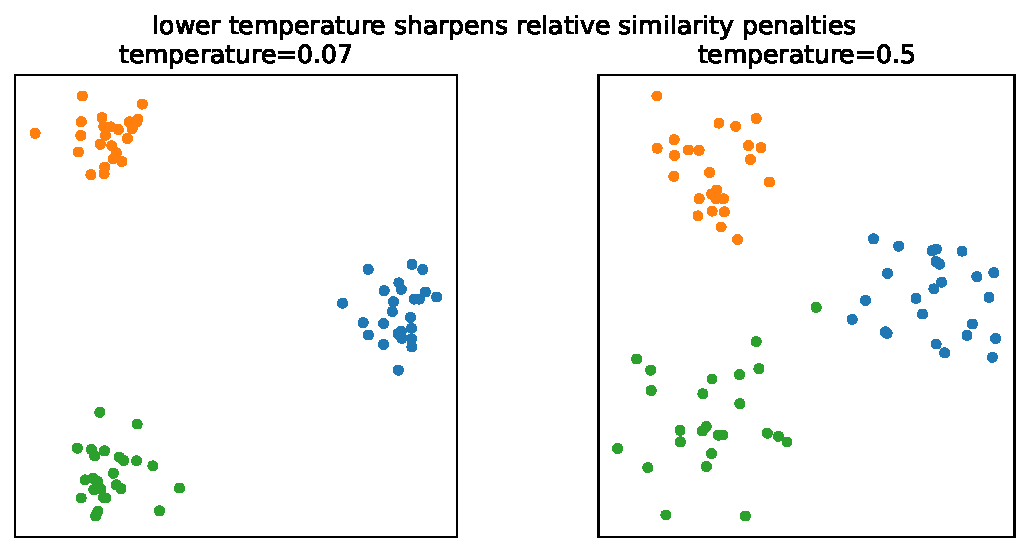
\includegraphics[width=0.9\textwidth]{fig11_11_contrastive.pdf}
\caption{نمای مفهومی هندسه کنتراستی و اثر دما بر فشردگی نسبی خوشه‌ها.}
\label{fig:contrastivegeometry}
\end{figure}

\begin{figure}[H]
\centering
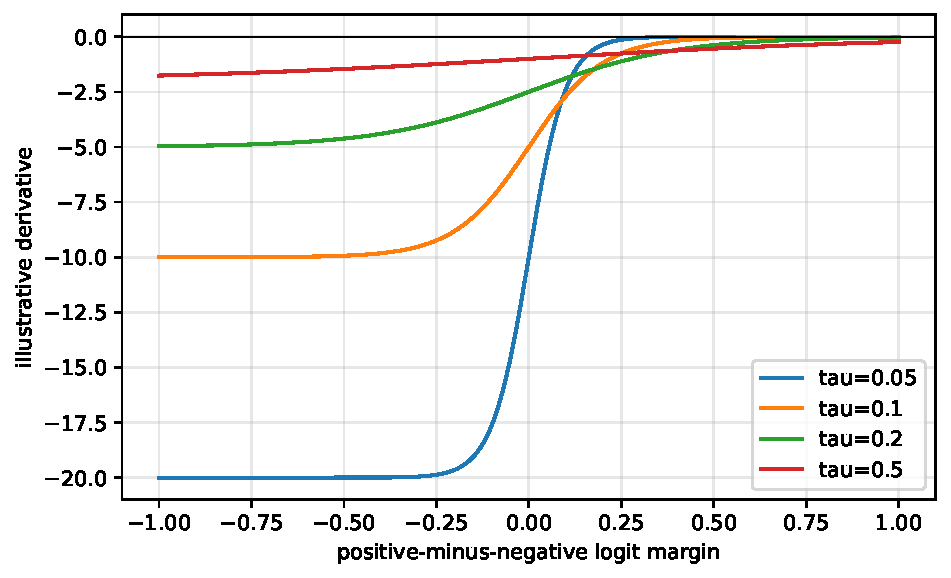
\includegraphics[width=0.76\textwidth]{fig11_12_temperature.pdf}
\caption{نمونه آموزشی اثر دما بر مشتق margin. دمای پایین حساسیت را زیاد می‌کند، اما پایداری و false negative را دشوارتر می‌سازد.}
\label{fig:temperature}
\end{figure}

\subsection{alignment و uniformity}
دو فشار هندسی در روش کنتراستی وجود دارد:
\begin{enumerate}
\item \textbf{هم‌ترازی:} نمایش دو نمای یک نمونه نزدیک شود؛
\item \textbf{پراکندگی:} نمایش نمونه‌های متفاوت روی کره collapse نکند.
\end{enumerate}
یک معیار هم‌ترازی:
\begin{equation}
\mathcal L_{\mathrm{align}}=\E\norm{\vect z-\vect z^+}_2^2
\end{equation}
و معیار یکنواختی نمونه:
\begin{equation}
\mathcal L_{\mathrm{unif}}
=\log\E_{i\neq j}\exp(-t\norm{\vect z_i-\vect z_j}_2^2)
\end{equation}
است. loss پایین به‌تنهایی کافی نیست؛ ممکن است augmentation یا مجموعه negativeها وظیفه‌ای بسازد که با انتقال پایین‌دست ناسازگار باشد.

\subsection{ارتباط با کران اطلاعات متقابل و احتیاط لازم}
InfoNCE در شرایط خاص کران پایینی برای اطلاعات متقابل میان نماها فراهم می‌کند. برای $K$ نمونه در dictionary، شکلی از رابطه
\begin{equation}
I(X;Y)\geq \log K-\mathcal L_{\mathrm{NCE}}
\end{equation}
به دست می‌آید. اما این رابطه نباید به ادعای ساده «کمینه‌کردن loss یعنی بیشینه‌کردن تمام اطلاعات مفید» تبدیل شود. نوع score، توزیع negative، ظرفیت critic و augmentation تعیین می‌کنند چه اطلاعاتی باقی بماند. در عمل هدف، اطلاعات متقابل خام پیکسل نیست؛ ناوردایی کنترل‌شده و انتقال‌پذیری است.

\subsection{SimCLR}
\lr{SimCLR} نشان داد ترکیب augmentation قوی، projection head غیرخطی، batch بزرگ و آموزش طولانی می‌تواند بدون memory bank نمایش قدرتمند بسازد. خط لوله:
\begin{equation}
\vect x\xrightarrow{t_1,t_2}
\widetilde{\vect x}^{(1)},\widetilde{\vect x}^{(2)}
\xrightarrow{f_\theta}
\vect h^{(1)},\vect h^{(2)}
\xrightarrow{g_\phi}
\vect z^{(1)},\vect z^{(2)}.
\end{equation}
Batch بزرگ تعداد negative را زیاد می‌کند، اما نیاز حافظه و حساسیت به distributed all-gather را افزایش می‌دهد. اگر embedding از همه GPUها جمع می‌شود، gradient و ordering positiveها باید درست مدیریت شود.

\begin{workshopbox}[پیاده‌سازی InfoNCE و یک گام SimCLR]
\begin{latin}
\lstinputlisting{code/info_nce.py}
\lstinputlisting[firstline=1,lastline=48]{code/simclr_minimal.py}
\end{latin}
این کد آموزشی augmentation محدودی دارد. برای پژوهش واقعی، \lr{torchvision.transforms.v2} یا \lr{Kornia}، ثبت پارامتر تبدیل و آزمون دامنه‌ای لازم است.
\end{workshopbox}

\subsection{MoCo: dictionary پویا و encoder تکانه‌ای}
\lr{MoCo} صفی از keyهای batchهای گذشته می‌سازد تا dictionary بزرگ بدون batch عظیم به دست آید. encoder کلید با EMA به‌روزرسانی می‌شود:
\begin{equation}
\theta_k\leftarrow m\theta_k+(1-m)\theta_q.
\label{eq:moco-ema}
\end{equation}
اگر $m$ کوچک باشد، keyهای صف سریع ناسازگار می‌شوند؛ اگر بسیار نزدیک یک باشد، معلم دیر سازگار می‌شود. صف باید first-in-first-out باشد و keyهای جاری پس از محاسبه loss وارد شوند. در نسخه‌های بعد، recipe و backbone ViT نقش بیشتری پیدا کردند.

\subsection{false negative و داده با ساختار گروهی}
در batch، دو تصویر متفاوت ممکن است یک کلاس یا هویت معنایی داشته باشند و به‌اشتباه negative شوند. در داده پزشکی، دو crop از یک بیمار یا دو فریم نزدیک یک ویدئو نمونه آشکار است. راهکارها شامل metadata-aware sampling، حذف negativeهای مشکوک، supervised contrastive در بخش برچسب‌دار، multi-positive و روش‌های بدون negative است. اما حذف negative بدون سازوکار دیگر می‌تواند collapse ایجاد کند.

\section{خوشه‌بندی آنلاین و SwAV}
\lr{SwAV} به‌جای مقایسه همه زوج‌ها، assignment دو نمای یک تصویر به prototypeها را سازگار می‌کند. اگر prototypeها ستون‌های $\mat C\in\R^{D\times K}$ باشند:
\begin{equation}
\vect p=\softmax(\mat C\trans\vect z/\tau).
\end{equation}
Assignment هدف $\vect q$ با قید استفاده متوازن از prototypeها و الگوریتم Sinkhorn--Knopp محاسبه می‌شود. loss cross-view:
\begin{equation}
\mathcal L=-\sum_k q_k^{(1)}\log p_k^{(2)}-
\sum_k q_k^{(2)}\log p_k^{(1)}.
\end{equation}
قید تعادل مانع می‌شود همه نمونه‌ها به یک prototype بروند، اما اگر داده واقعاً نامتوازن باشد، تعادل مصنوعی می‌تواند ساختار طبیعی را تحریف کند.

\begin{algorithmbox}{الگوریتم مفهومی Sinkhorn برای assignment متوازن}
\begin{enumerate}
\item scoreهای prototype را نمایی کنید و ماتریس $\mat Q$ بسازید؛
\item چند بار سطرها را برای مجموع برابر $1/K$ نرمال کنید؛
\item ستون‌ها را برای مجموع برابر $1/B$ نرمال کنید؛
\item assignment نهایی را به مقیاس batch برگردانید؛
\item gradient از assignment teacher عبور ندهید.
\end{enumerate}
\end{algorithmbox}

\section{روش‌های بدون negative صریح: BYOL، SimSiam و DINO}
\subsection{BYOL و نقش عدم تقارن}
در \lr{BYOL}، شبکه online شامل encoder، projector و predictor است؛ شبکه target encoder و projector دارد و با EMA به‌روزرسانی می‌شود. loss نمونه پس از نرمال‌سازی:
\begin{equation}
\mathcal L_{\mathrm{BYOL}}
=2-2\frac{\vect q_\theta(\vect z_1)\trans\vect z_2^{\mathrm{target}}}
{\norm{\vect q_\theta(\vect z_1)}\norm{\vect z_2^{\mathrm{target}}}}
+\text{sym.}
\end{equation}
stop-gradient روی target و predictor تنها در شاخه online، تقارن کامل را می‌شکند. توضیح دقیق ضد collapse هنوز به optimization، normalization و معماری وابسته است؛ بیان اینکه «EMA به‌تنهایی مانع collapse است» بیش‌ازحد ساده است.

\subsection{SimSiam}
\lr{SimSiam} نشان داد حتی بدون encoder تکانه‌ای نیز stop-gradient و predictor می‌توانند کافی باشند. این نتیجه اهمیت دینامیک بهینه‌سازی و عدم تقارن را برجسته کرد. در پیاده‌سازی، گذاشتن stop-gradient در محل اشتباه یا حذف predictor می‌تواند رفتار را تغییر دهد.

\subsection{DINO: خودتقطیر با centering و sharpening}
در \lr{DINO}، دانش‌آموز چند crop و معلم معمولاً cropهای سراسری را می‌بیند. توزیع دانش‌آموز:
\begin{equation}
p_s^{(k)}(x)=
\frac{\exp(g_s(x)^{(k)}/\tau_s)}{\sum_{k'}\exp(g_s(x)^{(k')}/\tau_s)},
\end{equation}
و معلم با center $\vect c$:
\begin{equation}
p_t^{(k)}(x)=
\frac{\exp((g_t(x)^{(k)}-c_k)/\tau_t)}
{\sum_{k'}\exp((g_t(x)^{(k')}-c_{k'})/\tau_t)}.
\end{equation}
loss، cross-entropy خروجی معلم و دانش‌آموز روی نماهای متفاوت است. $\tau_t$ کوچک sharpening ایجاد می‌کند؛ center با میانگین متحرک به‌روزرسانی می‌شود تا یک یا چند بعد غالب نشوند. معلم با EMA وزن‌ها ساخته می‌شود.

\begin{figure}[H]
\centering
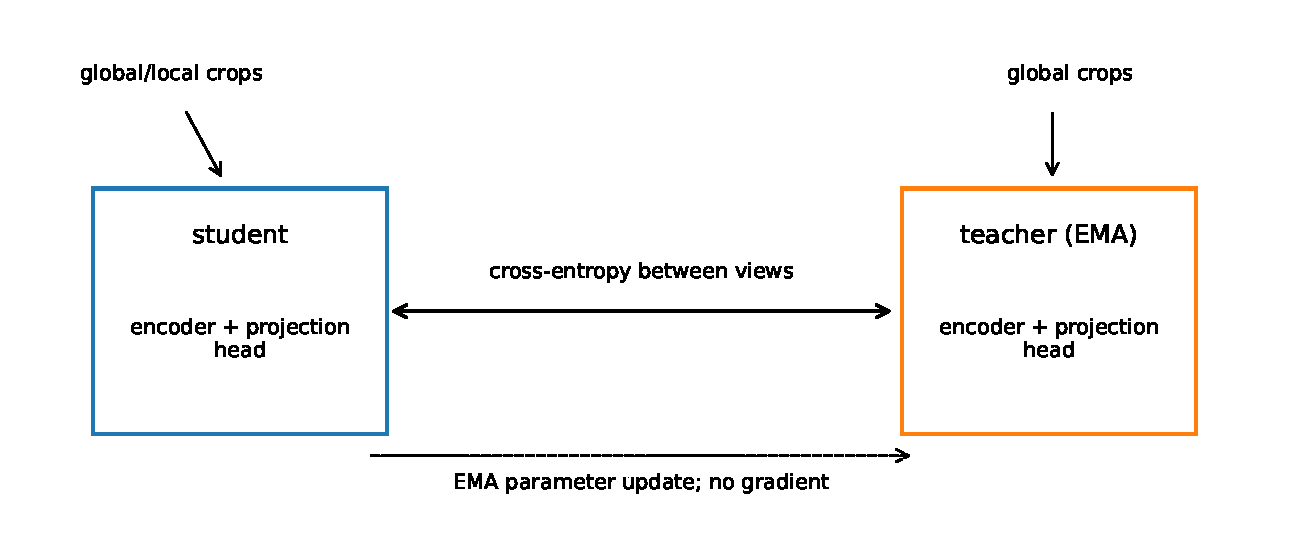
\includegraphics[width=0.93\textwidth]{fig11_18_dino.pdf}
\caption{ساختار teacher--student در DINO. gradient تنها به دانش‌آموز می‌رسد و معلم با EMA تغییر می‌کند.}
\label{fig:dino}
\end{figure}

\begin{figure}[H]
\centering
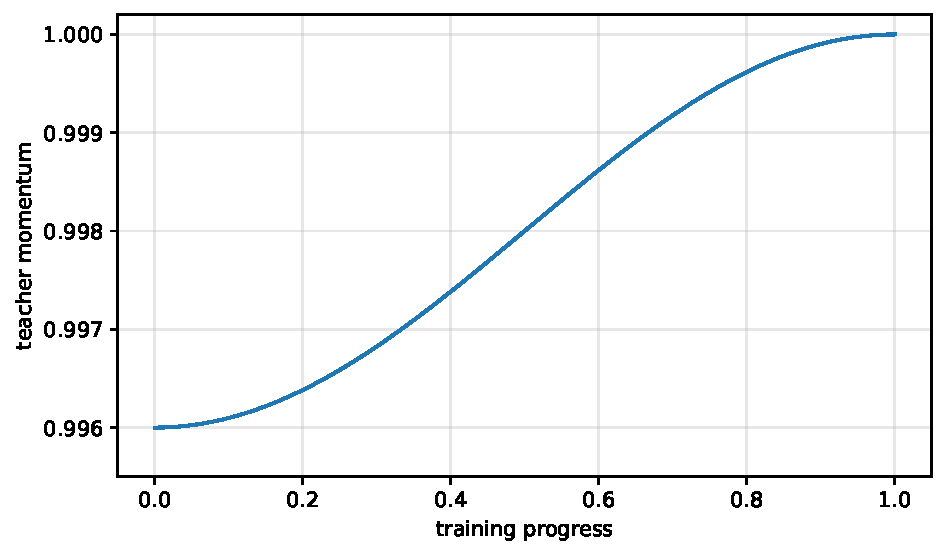
\includegraphics[width=0.73\textwidth]{fig11_15_ema.pdf}
\caption{schedule نمونه برای افزایش momentum معلم به سمت یک. مقدار دقیق باید با batch، طول آموزش و مدل هماهنگ شود.}
\label{fig:ema}
\end{figure}

\begin{workshopbox}[معلم EMA و loss تقطیر]
\begin{latin}
\lstinputlisting{code/dino_ema.py}
\end{latin}
نسخه کامل DINO به multi-crop، centering توزیع‌شده، schedule دمای معلم، weight normalization سر و هماهنگی EMA میان پردازش‌ها نیاز دارد.
\end{workshopbox}

\subsection{چرا ویژگی‌های متراکم در DINO مهم شدند؟}
در ViT خودنظارتی، patch tokenها بدون برچسب پیکسلی می‌توانند مرز و جزء معنایی را آشکار کنند. این خاصیت سبب شد backboneهای DINO برای قطعه‌بندی، تطبیق، عمق، بازیابی و correspondence به‌کار روند. با این حال، کیفیت dense feature باید با benchmark متراکم سنجیده شود؛ دقت kNN روی CLS تضمین‌کننده مرز دقیق نیست.

\section{کاهش افزونگی: Barlow Twins و VICReg}
\subsection{Barlow Twins}
دو batch embedding استانداردشده $\mat Z^A,\mat Z^B\in\R^{B\times D}$ داریم. ماتریس همبستگی متقاطع:
\begin{equation}
C_{ij}=\frac{\sum_b Z^A_{bi}Z^B_{bj}}
{\sqrt{\sum_b(Z^A_{bi})^2}\sqrt{\sum_b(Z^B_{bj})^2}}.
\end{equation}
تابع هدف:
\begin{equation}
\mathcal L_{\mathrm{BT}}
=\sum_i(1-C_{ii})^2+\lambda\sum_{i\neq j}C_{ij}^2.
\label{eq:barlow}
\end{equation}
قطر، ناوردایی دو نما را تحمیل می‌کند و خارج قطر، افزونگی ابعاد را کاهش می‌دهد. استانداردسازی batch بخش مهم objective است؛ batch کوچک تخمین همبستگی را پرنویز می‌کند.

\subsection{VICReg}
\lr{VICReg} سه جمله را صریح می‌کند. جمله ناوردایی:
\begin{equation}
s(\mat Z^A,\mat Z^B)=\frac{1}{B}\sum_b\norm{\vect z_b^A-\vect z_b^B}_2^2.
\end{equation}
جمله واریانس برای هر شاخه:
\begin{equation}
v(\mat Z)=\frac{1}{D}\sum_j\max\left(0,\gamma-\sqrt{\Var(Z_{:j})+\epsilon}\right).
\end{equation}
جمله کوواریانس:
\begin{equation}
c(\mat Z)=\frac{1}{D}\sum_{i\neq j}\Cov(\mat Z)_{ij}^2.
\end{equation}
و loss:
\begin{equation}
\mathcal L_{\mathrm{VICReg}}=\lambda s+\mu[v(\mat Z^A)+v(\mat Z^B)]
+\nu[c(\mat Z^A)+c(\mat Z^B)].
\label{eq:vicreg}
\end{equation}
جمله واریانس جلوی collapse هر بعد را می‌گیرد؛ جمله کوواریانس ابعاد تکراری را کاهش می‌دهد. hyperparameterها مقیاس سه جمله را متعادل می‌کنند و باید جداگانه log شوند.

\begin{keybox}[مقایسه ضد فروپاشی]
\begin{itemize}
\item \lr{InfoNCE}: رقابت positive با negativeها؛
\item \lr{SwAV}: assignment متوازن به prototypeها؛
\item \lr{BYOL/SimSiam}: عدم تقارن، predictor و stop-gradient؛
\item \lr{DINO}: teacher EMA، centering و sharpening؛
\item \lr{Barlow Twins}: همانی‌کردن همبستگی متقاطع؛
\item \lr{VICReg}: کران پایین واریانس و جریمه کوواریانس؛
\item \lr{MAE}: هدف بازسازی غیرثابت برای هر تصویر و mask.
\end{itemize}
\end{keybox}

\section{فروپاشی نمایش و ابزارهای تشخیص}
\subsection{فروپاشی کامل و فروپاشی بعدی}
در collapse کامل:
\begin{equation}
f_\theta(x)=\vect c\qquad\forall x.
\end{equation}
اما collapse می‌تواند جزئی باشد: embeddingها تنها در زیرفضای کم‌بعد تغییر کنند. اگر ماتریس centered embedding برابر $\mat Z_c$ و مقادیر ویژه کوواریانس $\lambda_1\geq\cdots\geq\lambda_D$ باشند، rank مؤثر:
\begin{equation}
r_{\mathrm{eff}}=\exp\left(-\sum_i p_i\log p_i\right),
\qquad
p_i=\frac{\lambda_i}{\sum_j\lambda_j}
\end{equation}
است. همچنین می‌توان تعداد ابعادی را که درصد مشخصی از انرژی را توضیح می‌دهند گزارش کرد.

\begin{figure}[H]
\centering
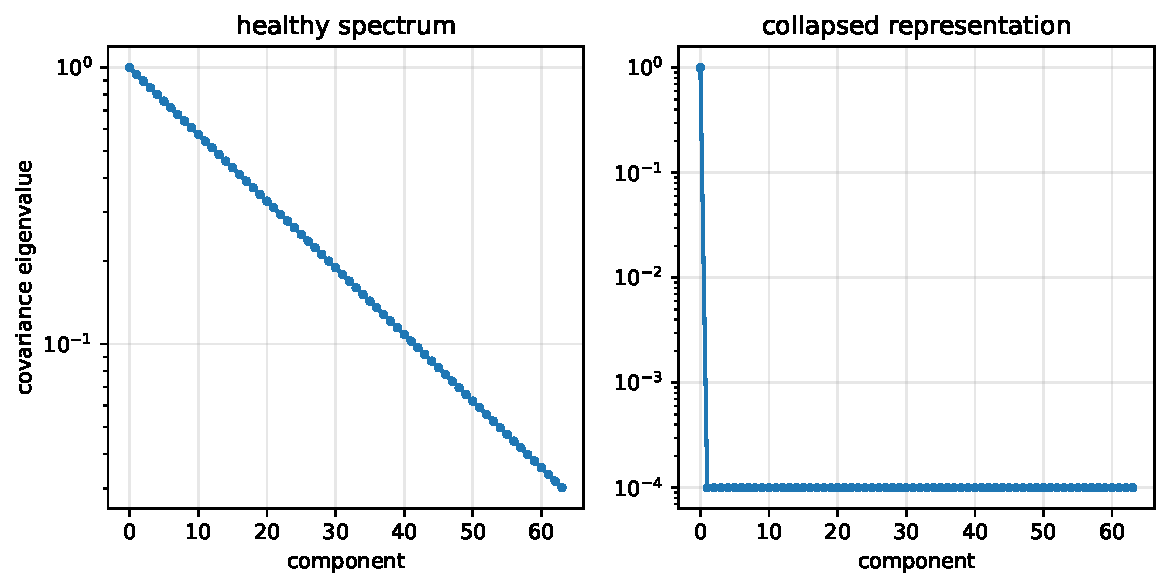
\includegraphics[width=0.9\textwidth]{fig11_14_collapse.pdf}
\caption{طیف کوواریانس سالم و فروپاشیده. فقط norm متوسط embedding برای تشخیص collapse کافی نیست.}
\label{fig:collapse}
\end{figure}

\subsection{چک‌لیست پایش در آموزش}
\begin{enumerate}
\item انحراف معیار هر بعد embedding و کمینه آن؛
\item spectrum کوواریانس و rank مؤثر؛
\item entropy خروجی teacher/student؛
\item norm گرادیان projector و backbone؛
\item میانگین شباهت positive و negative؛
\item histogram assignment prototype؛
\item lossهای جداگانه واریانس/کوواریانس/ناوردایی؛
\item kNN یا linear probe سبک روی snapshotهای دوره‌ای.
\end{enumerate}
Loss ثابت یا کاهش‌یابنده می‌تواند هم‌زمان با فروپاشی رخ دهد؛ diagnostic باید مستقیماً هندسه نمایش را بسنجد.

\section{مدل‌سازی ماسک‌شده تصویر}
\subsection{صورت‌بندی عمومی}
مجموعه شاخص توکن‌ها $\Omega=\{1,\ldots,N\}$ را به visible و masked تقسیم می‌کنیم:
\begin{equation}
\Omega=\mathcal V\cup\mathcal M,
\qquad
\mathcal V\cap\mathcal M=\varnothing.
\end{equation}
مدل از $x_{\mathcal V}$ هدف $y_{\mathcal M}$ را پیش‌بینی می‌کند:
\begin{equation}
\widehat y_{\mathcal M}=g_\phi(f_\theta(x_{\mathcal V}),\mathcal M).
\end{equation}
تفاوت روش‌ها در تعریف $y$، نسبت و شکل mask، معماری decoder و محل اعمال loss است.

\subsection{BEiT و هدف گسسته}
\lr{BEiT} تصویر را دو بار می‌بیند: وصله‌های پیوسته برای encoder و توکن‌های گسسته حاصل از tokenizer خارجی برای هدف. اگر $q_i\in\{1,\ldots,K\}$ کد وصله $i$ باشد:
\begin{equation}
\mathcal L_{\mathrm{BEiT}}
=-\sum_{i\in\mathcal M}\log p_\theta(q_i\mid x_{\mathcal V}).
\end{equation}
مزیت، هدف طبقه‌بندی معنایی‌تر از regression پیکسل است؛ ضعف، وابستگی به tokenizer و pipeline چندمرحله‌ای. اگر tokenizer بافت یا رنگی را کد کند که برای وظیفه هدف نامطلوب است، encoder همان bias را می‌آموزد.

\subsection{MAE و بازسازی پیکسل}
\lr{MAE} فقط توکن‌های visible را وارد encoder سنگین می‌کند. سپس latentها با mask tokenها به ترتیب اصلی بازگردانده و decoder سبک پیکسل وصله‌های masked را بازسازی می‌کند. برای وصله $i$:
\begin{equation}
\mathcal L_{\mathrm{MAE}}
=\frac{1}{\abs{\mathcal M}}\sum_{i\in\mathcal M}
\norm{\widehat{\vect x}_i-\vect x_i}_2^2.
\label{eq:mae}
\end{equation}
اغلب target هر وصله نرمال می‌شود:
\begin{equation}
\widetilde{\vect x}_i=\frac{\vect x_i-\mu_i}{\sqrt{\sigma_i^2+\epsilon}},
\end{equation}
تا مدل کمتر روی روشنایی مطلق و بیشتر روی ساختار تمرکز کند.

نسبت mask بالا مانند $75\%$ دو اثر دارد: وظیفه را دشوار و redundancy محلی را کم می‌کند؛ و encoder را ارزان می‌سازد چون فقط $25\%$ توکن‌ها را می‌بیند. اگر نسبت خیلی پایین باشد، interpolation محلی ساده کافی است؛ اگر بسیار بالا باشد، context برای ساختار ظریف ناکافی می‌شود.

\begin{figure}[H]
\centering
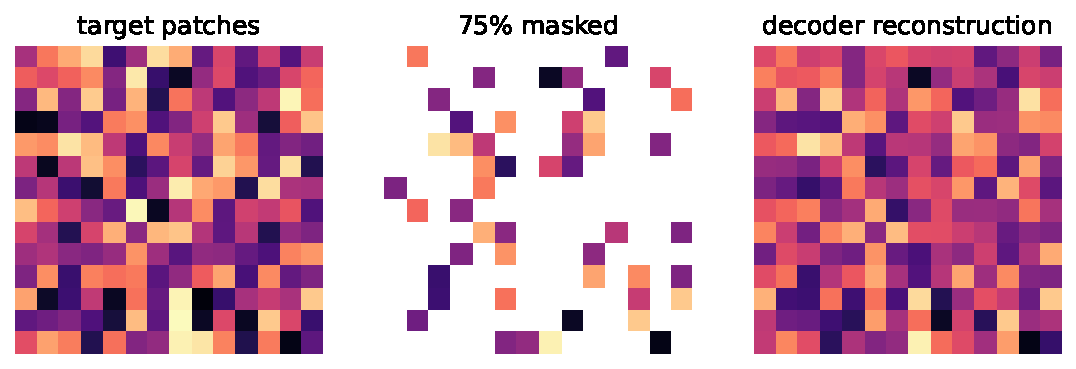
\includegraphics[width=0.87\textwidth]{fig11_16_mae.pdf}
\caption{ساختار مفهومی MAE با mask زیاد و decoder بازسازی. شکل داده مصنوعی است.}
\label{fig:mae}
\end{figure}

\begin{workshopbox}[MAE آموزشی]
\begin{latin}
\lstinputlisting{code/mae_minimal.py}
\end{latin}
این نسخه برای سادگی positional embedding ندارد. در مدل واقعی، ترتیب توکن visible، restoration index، embedding مکان encoder و decoder و mask schedule باید با دقت کنترل شوند.
\end{workshopbox}

\subsection{SimMIM}
\lr{SimMIM} نشان داد طراحی ساده mask و سر prediction سبک می‌تواند مؤثر باشد. پیام روش‌شناختی آن است که پیچیدگی tokenizer یا decoder همیشه ضروری نیست؛ اما نوع backbone، اندازه patch و normalization target نتیجه را تغییر می‌دهند.

\subsection{iBOT: tokenizer آنلاین}
\lr{iBOT} معلم را به tokenizer آنلاین تبدیل می‌کند. self-distillation هم روی token جهانی و هم patch token masked اعمال می‌شود. در نتیجه هدف محلی هم‌زمان با encoder تکامل می‌یابد و pipeline tokenizer جدا حذف می‌شود. اما ثبات معلم، centering و schedule mask پیچیده‌تر می‌گردد.

\subsection{data2vec: هدف contextualized latent}
\lr{data2vec} student ورودی masked را می‌بیند و نمایش contextualized معلم از ورودی کامل را پیش‌بینی می‌کند. اگر $\vect y_i$ میانگین یا ترکیب چند لایه معلم باشد:
\begin{equation}
\mathcal L=\sum_{i\in\mathcal M}\rho(\widehat{\vect y}_i-\vect y_i),
\end{equation}
که $\rho$ می‌تواند smooth $L_1$ باشد. هدف نه کد گسسته و نه پیکسل است؛ context کامل معلم را فشرده می‌کند.

\begin{figure}[H]
\centering
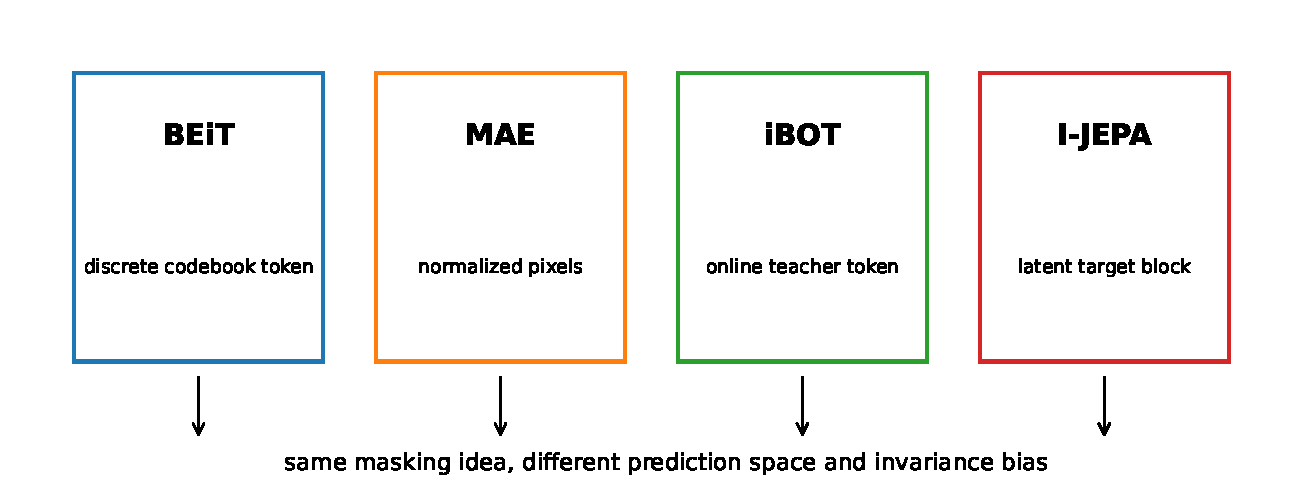
\includegraphics[width=0.96\textwidth]{fig11_17_targets.pdf}
\caption{فضاهای هدف متفاوت در مدل‌سازی ماسک‌شده و پیش‌بینی نهفته. انتخاب target نوع اطلاعات آموخته‌شده را تعیین می‌کند.}
\label{fig:targets}
\end{figure}

\subsection{شکل mask}
mask مستقل تصادفی، بلوکی، چندمقیاسی یا معنایی می‌تواند استفاده شود. mask تصادفی coverage یکنواخت دارد؛ mask بلوکی context دوربرد و ساختار کلان را می‌آزماید؛ mask معنایی خطر leakage از detector یا مدل قبلی دارد. برای داده پزشکی سه‌بعدی، mask مکعبی ممکن است ضایعه کوچک را کامل حذف کند و هدف بسیار مبهم شود.

\begin{keybox}[چه چیزی را بازسازی کنیم؟]
\begin{itemize}
\item پیکسل: دقیق و ساده، اما حساس به جزئیات کم‌اهمیت؛
\item پیکسل نرمال‌شده: بافت و ساختار نسبی؛
\item توکن گسسته: هدف طبقه‌بندی، وابسته به codebook؛
\item ویژگی teacher: هدف معنایی‌تر، وابسته به کیفیت و collapse معلم؛
\item feature چندمقیاسی: انتقال dense بهتر، هزینه حافظه بیشتر.
\end{itemize}
\end{keybox}

\section{I-JEPA و پیش‌بینی در فضای نهفته}
\lr{I-JEPA} از یک context block، نمایش چند target block را پیش‌بینی می‌کند. encoder context تنها پیکسل‌های context را می‌بیند؛ encoder target از تصویر کامل یا targetها نمایش می‌سازد و با EMA به‌روزرسانی می‌شود. predictor موقعیت target را نیز دریافت می‌کند:
\begin{equation}
\widehat{\vect y}_{\mathcal T}
=p_\phi(f_\theta(x_{\mathcal C}),\operatorname{pos}(\mathcal T)).
\end{equation}
loss نمونه:
\begin{equation}
\mathcal L_{\mathrm{JEPA}}
=\frac{1}{\abs{\mathcal T}}\sum_{i\in\mathcal T}
\norm{\widehat{\vect y}_i-\operatorname{sg}(\vect y_i^{\mathrm{target}})}_1.
\end{equation}
هدف این است که مدل جزئیات غیرقابل‌پیش‌بینی پیکسل را نادیده بگیرد و ساختار سطح بالاتر را پیش‌بینی کند.

\subsection{چرا sampling بلوک مهم است؟}
اگر target بسیار کوچک باشد، texture محلی کافی است؛ اگر context بسیار بزرگ و target نزدیک باشد، copy یا interpolation ممکن است؛ اگر context خیلی کوچک باشد، هدف غیرقابل پیش‌بینی است. در I-JEPA targetهای نسبتاً بزرگ و context فضایی توزیع‌شده، مدل را به semantics سوق می‌دهد. بنابراین masking تنها حذف داده نیست، طراحی سطح دشواری و نوع اطلاعات است.

\subsection{JEPA در برابر MAE}
\begin{longtable}{p{31mm}p{51mm}p{51mm}}
\toprule
ویژگی & MAE & I-JEPA \\
\midrule
فضای هدف & پیکسل/وصله & embedding معلم \\
decoder/predictor & decoder بازسازی & predictor نهفته \\
جزئیات تصادفی & باید تا حدی بازسازی شود & می‌تواند نادیده گرفته شود \\
ضد collapse & هدف پیکسل متغیر & target encoder EMA + طراحی predictor \\
حساسیت کلیدی & mask ratio و target normalization & sampling context/target و کیفیت target \\
کاربرد طبیعی & پیش‌آموزش عمومی و بازسازی & نمایش معنایی و پیش‌بینی \\
\bottomrule
\end{longtable}

\section{مدل‌های بنیادی خودنظارتی}
\subsection{DINOv2: روش، داده و مهندسی مقیاس}
\lr{DINOv2} تنها یک loss جدید نیست؛ ترکیبی از self-distillation، masked patch objective، داده‌گزینی، training at scale و distillation به مدل‌های کوچک‌تر است. این نکته برای دانشجو مهم است: در مقیاس بنیادین، کیفیت داده، deduplication، balancing، schedule و pipeline توزیع‌شده بخشی از الگوریتم‌اند.

برای ارزیابی ویژگی عمومی، باید وظایف جهانی و متراکم جدا شوند: kNN/linear classification، retrieval، segmentation، depth، correspondence و robustness. یک مدل ممکن است CLS قوی اما patch feature ضعیف یا برعکس داشته باشد.

\subsection{register tokenها}
در ViT بزرگ، بعضی patch tokenها ممکن است به نقش storage جهانی تبدیل و norm غیرعادی پیدا کنند. register tokenهای آموختنی فضای جدا برای این نقش فراهم می‌کنند تا patch tokenها مکانی‌تر بمانند. registerها خروجی مکانی مستقیم ندارند و در decoder dense باید جدا شوند.

\subsection{DINOv3 و مقیاس جدید}
\lr{DINOv3} مسیر self-supervised foundation backbone را به مقیاس بزرگ‌تر ادامه می‌دهد و بر کیفیت dense feature، سازگاری وضوح و انتقال بدون fine-tuning تأکید دارد. recipe رسمی شامل مرحله پیش‌آموزش، پالایش ساختار نمایش و سازگاری وضوح بالا است. در تدریس باید میان سه سطح تمایز گذاشت:
\begin{enumerate}
\item objective بنیادی teacher--student؛
\item recipe مقیاس و داده؛
\item post-hoc adaptation و distillation.
\end{enumerate}
بازسازی کامل چنین مدل‌هایی در کلاس ممکن نیست، اما استخراج ویژگی، linear probe، dense correspondence و تحلیل resolution قابل انجام است.

\subsection{EVA-02}
\lr{EVA-02} از masked image modeling برای بازسازی ویژگی‌های یک teacher هم‌تراز با زبان استفاده می‌کند. این روش مرز میان self-supervised بصری و distillation از مدل vision-language را کمرنگ می‌کند. target قوی می‌تواند semantics را منتقل کند، اما bias و محدودیت teacher نیز منتقل می‌شود.

\section{پیش‌آموزش تصویر ـ متن: CLIP، SigLIP و SigLIP 2}
گرچه نظارت طبیعی متن کاملاً «بدون برچسب» نیست، این خانواده برای فهم مدل‌های بنیادی ضروری است. یک encoder تصویر $f$ و encoder متن $g$ embedding نرمال‌شده می‌سازند. در \lr{CLIP}، loss کنتراستی دوطرفه روی ماتریس شباهت batch اعمال می‌شود:
\begin{equation}
S_{ij}=\frac{f(x_i)\trans g(t_j)}{\tau}.
\end{equation}
\begin{equation}
\mathcal L_{\mathrm{CLIP}}
=\frac12\left[\CE(S,\operatorname{diag})+\CE(S\trans,\operatorname{diag})\right].
\end{equation}
متن فضای مفهومی باز و zero-shot classification را فراهم می‌کند، اما caption ممکن است مکان، شمارش یا جزئیات ریز را پوشش ندهد.

\subsection{SigLIP}
\lr{SigLIP} به‌جای softmax سراسری، loss sigmoid زوجی استفاده می‌کند. اگر $y_{ij}=+1$ برای زوج صحیح و $-1$ برای زوج نادرست:
\begin{equation}
\mathcal L_{\mathrm{sig}}
=\sum_{i,j}\log\left(1+\exp[-y_{ij}(s_{ij}+b)]\right).
\end{equation}
این objective وابستگی normalization به کل batch را کاهش می‌دهد و scaling batch را تغییر می‌دهد.

\subsection{SigLIP 2}
\lr{SigLIP 2} loss زبان ـ تصویر را با captioning-based pretraining، self-distillation، masked prediction و data curation ترکیب می‌کند. نسخه‌های چندوضوح و حفظ نسبت تصویر نشان می‌دهند توکن‌سازی بومی و self-supervision اکنون بخشی از recipe مدل چندوجهی‌اند. ویژگی متراکم قوی برای localization نیز اهمیت دارد.

\begin{futurebox}
مرز میان «مدل بصری خودنظارتی»، «مدل تصویر ـ متن» و «vision encoder مدل چندوجهی» در حال محو شدن است. فصل آینده باید مدل مولد و foundation model را بر اساس objective، داده و interface تحلیل کند، نه صرفاً نام محصول.
\end{futurebox}

\section{انتقال نمایش به وظایف پایین‌دست}
\subsection{kNN و linear probe}
در kNN، backbone frozen است و شباهت embeddingها تصمیم را می‌سازد. اگر ویژگی‌ها نرمال باشند، cosine و ضرب داخلی هم‌ارزند. weighted kNN:
\begin{equation}
\operatorname{score}(c\mid z)=\sum_{i\in\mathcal N_k(z)}
\exp(s_i/\tau_{knn})\,\mathbb 1[y_i=c].
\end{equation}
Linear probe یک لایه خطی روی ویژگی frozen آموزش می‌دهد. این معیار separability خطی را می‌سنجد، نه ظرفیت کامل fine-tuning.

\subsection{fine-tuning کامل و لایه‌ای}
در fine-tuning کامل، نرخ یادگیری backbone معمولاً کمتر از head است. layer-wise learning-rate decay:
\begin{equation}
\eta_l=\eta_{\mathrm{top}}\alpha^{L-l},\qquad 0<\alpha<1
\end{equation}
لایه‌های پایین را محافظه‌کارتر تغییر می‌دهد. weight decay نباید روی bias و پارامترهای normalization بدون تصمیم آگاهانه اعمال شود. positional embedding و patch projection برای وضوح جدید نیازمند adaptation هستند.

\subsection{adapter، LoRA و prompt tuning}
برای ماتریس وزن $\mat W\in\R^{d_o\times d_i}$، \lr{LoRA} تغییر کم‌رتبه:
\begin{equation}
\Delta\mat W=\mat A\mat B,
\qquad
\mat A\in\R^{d_o\times r},\ \mat B\in\R^{r\times d_i},\ r\ll d
\end{equation}
می‌آموزد. adapter یک bottleneck residual به بلوک می‌افزاید و visual prompt توکن‌های آموختنی را به دنباله اضافه می‌کند. کاهش پارامتر trainable لزوماً کاهش حافظه activation یا latency نیست؛ benchmark باید end-to-end باشد.

\subsection{داده کم‌برچسب}
\begin{figure}[H]
\centering
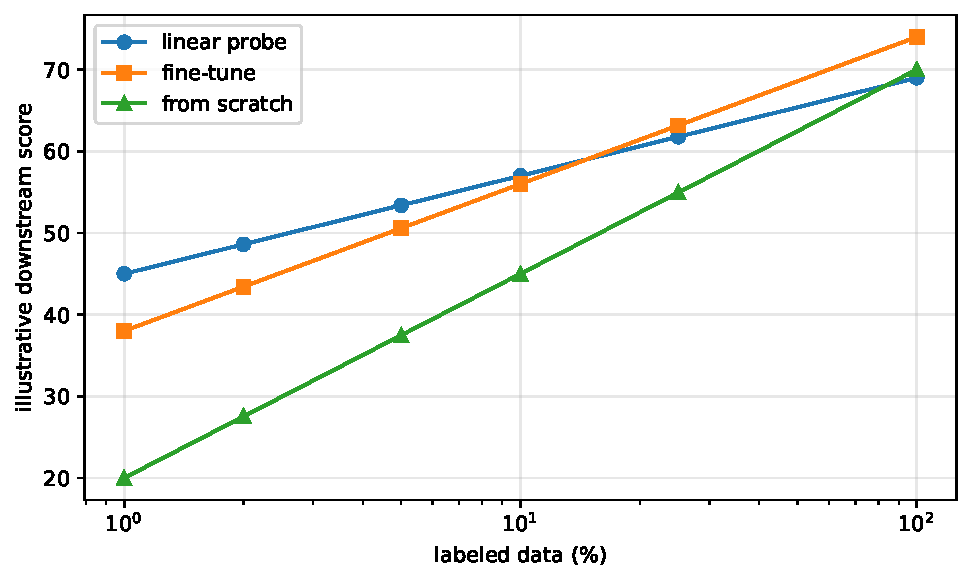
\includegraphics[width=0.78\textwidth]{fig11_22_transfer.pdf}
\caption{منحنی آموزشی نمونه برای مقایسه linear probe، fine-tuning و آموزش از صفر در نسبت‌های مختلف برچسب. اعداد واقعی نیستند.}
\label{fig:transfer}
\end{figure}

در داده بسیار کم، linear probe یا adapter می‌تواند overfitting را کم کند. با افزایش برچسب و domain shift، fine-tuning کامل سودمندتر می‌شود. انتخاب باید با منحنی label-efficiency، چند seed و فاصله اطمینان انجام شود.

\section{انتقال متراکم: از patch token تا نقشه ویژگی}
برای ViT با grid $H_p\times W_p$، patch tokenهای لایه $l$ را می‌توان به
\begin{equation}
\mat F_l\in\R^{H_p\times W_p\times D_l}
\end{equation}
بازشکل داد. decoder قطعه‌بندی یا عمق از یک یا چند لایه استفاده می‌کند. ViT ساده هرم طبیعی ندارد؛ راهکارها:
\begin{itemize}
\item projection چند لایه به مقیاس‌های مصنوعی؛
\item backbone سلسله‌مراتبی مانند Swin/Hiera؛
\item adapter کانولوشنی؛
\item feature pyramid decoder؛
\item استفاده از patch کوچک یا وضوح بالاتر.
\end{itemize}
در dense transfer، interpolation ویژگی و alignment مختصات باید با مرکز پیکسل، padding و stride سازگار باشد. خطای یک نیم‌پیکسل می‌تواند در مرزها مهم شود.

\subsection{correspondence و تطبیق با ویژگی خودنظارتی}
برای دو تصویر، patch featureهای نرمال $\mat F^A,\mat F^B$ ماتریس شباهت
\begin{equation}
\mat S=\mat F^A(\mat F^B)\trans
\end{equation}
می‌سازند. nearest neighbor اولیه باید با mutual check، هندسه، scale و occlusion پالایش شود. ویژگی dense DINO برای این کار مفید است، اما resolution و patch size حد دقت مکانی را تعیین می‌کنند.

\section{ارزیابی یک نمایش: یک عدد کافی نیست}
\begin{figure}[H]
\centering
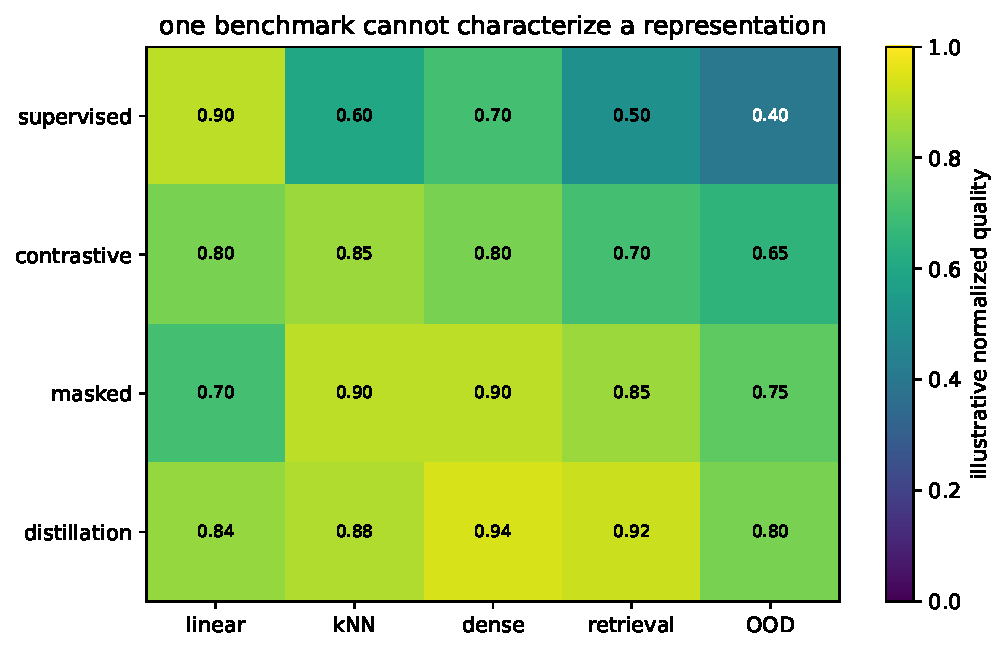
\includegraphics[width=0.8\textwidth]{fig11_24_evaluation.pdf}
\caption{یک objective می‌تواند در معیارهای جهانی و متراکم رفتار متفاوت داشته باشد؛ جدول فقط مفهوم چندمحوری‌بودن ارزیابی را نشان می‌دهد.}
\label{fig:evalmatrix}
\end{figure}

\subsection{پروتکل‌های اصلی}
\begin{enumerate}
\item \textbf{kNN:} بدون آموزش head پیچیده؛ حساس به normalization و $k$؛
\item \textbf{linear probe:} separability خطی؛ حساس به optimizer و epoch؛
\item \textbf{fine-tuning:} ظرفیت کامل انتقال؛ حساس به recipe؛
\item \textbf{few-shot:} منحنی عملکرد بر حسب برچسب؛
\item \textbf{retrieval:} Recall@K، mAP و deduplication؛
\item \textbf{dense transfer:} mIoU، AP، depth error و correspondence؛
\item \textbf{robustness:} corruption، shift، OOD و adversarial؛
\item \textbf{calibration:} NLL، Brier و ECE؛
\item \textbf{کارایی:} زمان پیش‌آموزش، انرژی، حافظه، latency و throughput.
\end{enumerate}

\subsection{پروتکل linear probe عادلانه}
backbone باید در حالت eval باشد؛ augmentation train و eval جدا؛ feature normalization مشخص؛ head و optimizer برای همه روش‌ها یکسان؛ و اگر ویژگی چند لایه یا pooling انتخاب می‌شود، انتخاب روی validation انجام شود. گزارش بهترین تنظیم برای یک مدل و تنظیم پیش‌فرض برای مدل دیگر مقایسه را مخدوش می‌کند.

\subsection{ارزیابی بدون نشت}
در داده بیمارمحور، ویدئویی یا مکانی، split باید در سطح هویت مستقل باشد. دو crop از یک تصویر یا فریم‌های یک ویدئو در train/test نشت ایجاد می‌کنند. در self-supervised pretraining نیز overlap داده پیش‌آموزش با benchmark باید مستند شود، به‌ویژه برای مدل‌های وب‌مقیاس.

\subsection{عدم‌قطعیت و OOD}
feature قوی به معنی اعتماد درست نیست. head خطی می‌تواند overconfident باشد. علاوه بر accuracy، entropy، energy score، Mahalanobis distance، calibration و performance روی domain shift سنجیده شود. مدل بنیادی ممکن است در داده طبیعی عالی و در modality تخصصی فاقد اطلاعات رنگ/هندسه مناسب باشد.

\section{کتابخانه‌ها: از kernel تا recipe خودنظارتی}
\begin{figure}[H]
\centering
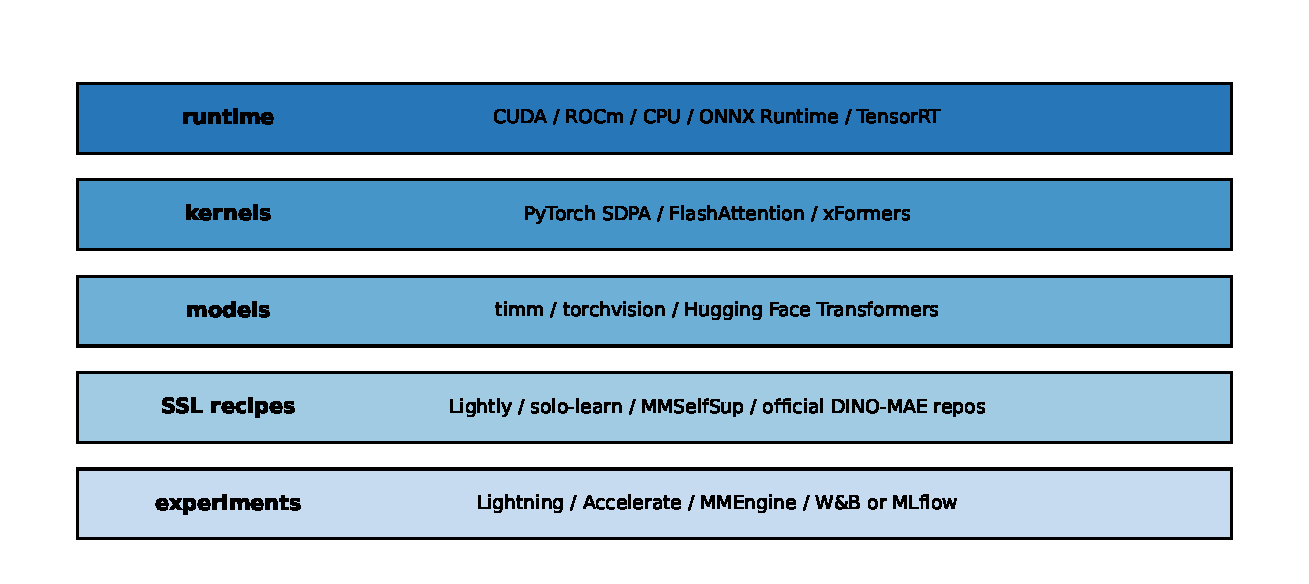
\includegraphics[width=0.94\textwidth]{fig11_23_libraries.pdf}
\caption{لایه‌های ابزار. انتخاب library باید بر اساس سطح انتزاع و نیاز بازتولیدپذیری باشد.}
\label{fig:libraries}
\end{figure}

\subsection{PyTorch}
برای آموزش از صفر، اجزای اصلی عبارت‌اند از:
\begin{itemize}
\item \lr{Conv2d} یا reshape برای patch embedding؛
\item \lr{LayerNorm} و \lr{Linear}؛
\item \lr{scaled\_dot\_product\_attention} برای kernel بهینه؛
\item \lr{DistributedDataParallel} برای چند GPU؛
\item \lr{autocast} و \lr{GradScaler} برای mixed precision؛
\item \lr{torch.compile} در صورت سازگاری graph و backend.
\end{itemize}
در SSL، all-gather embedding، synchronized BatchNorm/centering، queue و EMA نیازمند مدیریت توزیع‌شده‌اند.

\subsection{torchvision و timm}
\lr{torchvision} مدل‌ها، transforms و feature extraction رسمی PyTorch را فراهم می‌کند. \lr{timm} مجموعه گسترده‌تری از backboneها، وزن‌ها، augmentationها، optimizer و training script دارد. هنگام بارگذاری وزن:
\begin{enumerate}
\item preprocessing config را از خود وزن بخوانید؛
\item mean/std، interpolation، crop percentage و resolution را ثبت کنید؛
\item \lr{num\_classes=0} یا \lr{features\_only=True} را آگاهانه انتخاب کنید؛
\item نام checkpoint و revision را ثابت کنید.
\end{enumerate}

\subsection{Hugging Face Transformers}
این کتابخانه مدل‌های \lr{ViT}، \lr{ViTMAE}، \lr{BEiT}، \lr{DINOv2/v3}، \lr{I-JEPA}، \lr{Swin} و بسیاری encoderهای vision را با config و processor یکپارچه ارائه می‌کند. تفاوت \lr{AutoImageProcessor} با transform دستی باید روشن باشد؛ دو preprocessing متفاوت می‌توانند performance را تغییر دهند.

\subsection{Lightly، solo-learn و MMSelfSup}
این ابزارها recipeهای SSL را آماده می‌کنند:
\begin{itemize}
\item \lr{Lightly}: loss، transform و مثال‌های روش‌های کنتراستی و non-contrastive؛
\item \lr{solo-learn}: مجموعه پژوهشی روش‌های SSL برای مقایسه؛
\item \lr{MMSelfSup}: config-based training در اکوسیستم OpenMMLab؛
\item مخازن رسمی \lr{MAE} و \lr{DINOv2/v3}: مرجع جزئیات واقعی recipe.
\end{itemize}
استفاده از کتابخانه، مسئولیت فهم objective و config را حذف نمی‌کند. نسخه، commit و تغییرات محلی باید ثبت شوند.

\subsection{WebDataset و داده وب‌مقیاس}
برای میلیون‌ها تصویر، فایل‌های کوچک جداگانه bottleneck metadata ایجاد می‌کنند. shardهای tar، streaming، resampling و prefetch راهکار رایج‌اند. اما shuffle تقریبی، خرابی نمونه، deduplication و reproducibility دشوارتر می‌شود. شمار نمونه مؤثر هر epoch باید log شود.

\begin{librarybox}[مخازن رسمی به‌عنوان مشخصات اجرایی]
مقاله objective را توضیح می‌دهد، اما جزئیاتی مانند warm-up دما، schedule mask، teacher momentum، weight decay، gradient clipping و augmentation اغلب در config رسمی دقیق‌ترند. برای بازسازی، paper و repository باید با هم خوانده شوند؛ کپی config بدون فهم سخت‌افزار و batch نیز کافی نیست.
\end{librarybox}

\section{مهندسی آموزش در مقیاس}
\subsection{batch مؤثر و gradient accumulation}
اگر batch هر GPU برابر $B_g$، تعداد GPU برابر $G$ و تعداد گام accumulation برابر $A$ باشد:
\begin{equation}
B_{\mathrm{eff}}=B_gGA.
\end{equation}
اما accumulation دقیقاً معادل batch بزرگ نیست اگر BatchNorm، queue، teacher update یا schedule بر حسب step به‌روز شوند. در SSL کنتراستی، تعداد negativeهای هم‌زمان ممکن است تنها $B_gG$ باشد، نه $B_{\mathrm{eff}}$، مگر embedding چند microbatch ذخیره شود.

\subsection{EMA در آموزش توزیع‌شده}
تمام rankها باید دانش‌آموز یکسان داشته باشند؛ سپس teacher به‌صورت محلی با EMA به‌روزرسانی می‌شود. اگر stochastic operation یا optimizer state ناهمگام باشد، teacherها واگرا می‌شوند. center و prototype statistics نیز باید all-reduce شوند. checkpoint باید هر دو شبکه، center، optimizer، scaler و schedule progress را ذخیره کند.

\subsection{mixed precision}
در FP16، softmax logits و variance کوچک می‌توانند overflow/underflow کنند. BF16 دامنه exponent بزرگ‌تری دارد و برای transformer معمولاً پایدارتر است، اگر سخت‌افزار پشتیبانی کند. normalization و loss reduction ممکن است در FP32 اجرا شوند. نوع precision بخشی از recipe است و باید گزارش شود.

\subsection{weight decay و پارامترهای مستثنا}
در ViT معمولاً weight decay روی ماتریس‌های وزن اعمال می‌شود، اما bias، LayerNorm و گاهی positional/class/register tokenها مستثنا هستند. اگر مجموعه پارامترها به‌اشتباه ساخته شود، تغییر کوچک config می‌تواند نتیجه را جابه‌جا کند. کد باید نام و تعداد پارامتر هر گروه optimizer را چاپ کند.

\subsection{scheduleهای متداول}
نرخ یادگیری با batch مقیاس داده می‌شود، warm-up اولیه و cosine decay رایج‌اند:
\begin{equation}
\eta(t)=\eta_{\min}+\frac{1}{2}(\eta_{\max}-\eta_{\min})
\left[1+\cos\left(\pi\frac{t-t_w}{T-t_w}\right)\right].
\end{equation}
Teacher momentum، weight decay و دمای teacher نیز ممکن است schedule مستقل داشته باشند. نمایش فقط منحنی loss بدون نمایش scheduleها برای عیب‌یابی کافی نیست.

\subsection{checkpoint و بازتولیدپذیری}
یک checkpoint پژوهشی باید شامل موارد زیر باشد:
\begin{itemize}
\item وزن student و teacher؛
\item optimizer، scheduler و AMP scaler؛
\item epoch، global step و sampler state؛
\item center/prototype/queue؛
\item RNG stateهای Python، NumPy، CPU و CUDA؛
\item config resolved و commit کد؛
\item manifest داده یا shard list.
\end{itemize}
Resume از checkpoint باید با آزمون کوتاه بررسی شود که loss و schedule از همان نقطه ادامه می‌یابند.

\section{طراحی آزمایش‌های دقیق}
\subsection{آزمایش ۱: اندازه وصله}
مدل، داده و بودجه آموزش ثابت؛ $P\in\{8,16,32\}$. گزارش:
\begin{enumerate}
\item تعداد توکن و peak memory؛
\item throughput آموزش و inference؛
\item linear probe و fine-tuning؛
\item عملکرد شیء کوچک/بافت ریز؛
\item sensitivity به تغییر وضوح.
\end{enumerate}
اگر batch به‌دلیل حافظه تغییر می‌کند، optimizer و schedule باید برای مقایسه تنظیم یا این confound صریح گزارش شود.

\subsection{آزمایش ۲: کدگذاری مکان}
مقایسه embedding مطلق، relative bias و 2D RoPE روی آموزش 224 و ارزیابی 224، 384 و نسبت تصویر غیرمربع. معیارها: accuracy، calibration، dense localization و artefact مکانی. فقط interpolation موفق tensor به معنی تعمیم هندسی نیست.

\subsection{آزمایش ۳: دمای InfoNCE}
$\tau\in\{0.05,0.1,0.2,0.5\}$ با batch و augmentation ثابت. علاوه بر loss، similarity مثبت/منفی، norm گرادیان، rank مؤثر و linear probe را رسم کنید. بهترین loss ممکن است بهترین انتقال نباشد.

\subsection{آزمایش ۴: نسبت mask}
برای MAE نسبت $\{0.5,0.65,0.75,0.9\}$، زمان هر epoch، کیفیت reconstruction، linear probe و dense transfer را گزارش کنید. decoder capacity ثابت باشد. mask ratio بالا encoder را ارزان می‌کند، بنابراین مقایسه باید هم epoch ثابت و هم compute ثابت داشته باشد.

\subsection{آزمایش ۵: فضای هدف}
با backbone و داده یکسان، هدف پیکسل، پیکسل نرمال‌شده، feature teacher و token گسسته مقایسه شود. معیارهای جهانی و متراکم جدا گزارش شوند. این آزمایش نشان می‌دهد objective چه اطلاعاتی را ترجیح می‌دهد.

\subsection{آزمایش ۶: augmentation دامنه‌ای}
برای داده پزشکی/صنعتی، هر augmentation ابتدا از نظر فیزیکی توجیه و سپس ablation شود. جدول پیشنهادی:
\begin{longtable}{p{32mm}p{35mm}p{35mm}p{32mm}}
\toprule
تبدیل & ناوردایی مطلوب & خطر حذف سیگنال & آزمون تشخیصی \\
\midrule
crop & مکان و کادر & حذف ضایعه/عیب & overlap با ROI \\
color jitter & نورگیری & تغییر نشانگر رنگی & تحلیل کانال \\
blur & کیفیت حسگر & حذف بافت ریز & عملکرد بر حسب فرکانس \\
rotation & جهت دوربین & جهت تشخیصی & گروه‌بندی زاویه \\
flip & تقارن & چپ/راست معنایی & ارزیابی سمت \\
\bottomrule
\end{longtable}

\subsection{آزمایش ۷: پیش‌آموزش درون‌دامنه و برون‌دامنه}
سه initialization: random، مدل عمومی و SSL روی داده بدون برچسب دامنه. برای چند نسبت برچسب، منحنی عملکرد و فاصله اطمینان گزارش شود. اگر داده دامنه کم و یکنواخت است، SSL درون‌دامنه ممکن است overfit یا collapse کند؛ ترکیب داده عمومی و تخصصی بررسی شود.

\subsection{آزمایش ۸: token pruning/merging}
برای budgetهای مختلف، علاوه بر top-1، معیار dense و worst-group را گزارش کنید. latency واقعی روی سخت‌افزار هدف و batchهای 1 و بزرگ سنجیده شود. کاهش FLOPs ممکن است به scatter/gather نامنظم و کاهش اندک سرعت منجر شود.

\subsection{آزمایش ۹: frozen dense features}
یک decoder خطی یا بسیار سبک روی patch featureهای لایه‌های مختلف آموزش دهید. این آزمون نشان می‌دهد semantics محلی در کدام عمق ظاهر می‌شود. resolution و interpolation را ثابت نگه دارید.

\subsection{آزمایش ۱۰: ممیزی فروپاشی}
در یک اجرای عمداً ناپایدار، یکی از centering، variance term، stop-gradient یا negativeها حذف شود. loss، spectrum و rank مؤثر ثبت شود. این آزمایش آموزشی نشان می‌دهد چرا هر سازوکار وجود دارد.

\begin{researchbox}[حداقل جدول گزارش پیش‌آموزش]
\begin{longtable}{p{38mm}p{96mm}}
\toprule
مولفه & آنچه باید گزارش شود \\
\midrule
داده & تعداد نمونه، dedup، split، license، filtering، sampling \\
ورودی & resolution، aspect policy، patch، کانال، normalization \\
augmentation & ترتیب، احتمال و بازه پارامتر هر تبدیل \\
مدل & depth، width، heads، MLP ratio، position، registers \\
objective & loss کامل، وزن جمله‌ها، temperature، mask و target \\
teacher & momentum schedule، centering، update frequency \\
بهینه‌سازی & optimizer، lr، warm-up، decay، clipping، precision \\
توزیع & GPU، batch، accumulation، all-gather، sync statistics \\
هزینه & GPU-hours، energy در صورت امکان، peak memory \\
ارزیابی & kNN، linear، fine-tune، dense، robustness و variance seed \\
\bottomrule
\end{longtable}
\end{researchbox}

\section{عیب‌یابی سیستماتیک}
\begin{diagnosticbox}[loss خودنظارتی کم نمی‌شود]
\begin{enumerate}
\item positive mapping و ordering batch را بررسی کنید؛
\item normalization embedding و دما را چاپ کنید؛
\item augmentationها را تصویری ذخیره کنید؛
\item all-gather و label offset را در چند GPU بررسی کنید؛
\item learning rate و warm-up را نسبت به batch بازبینی کنید؛
\item gradient norm backbone و projector را جدا log کنید.
\end{enumerate}
\end{diagnosticbox}

\begin{diagnosticbox}[loss کم است اما linear probe ضعیف]
ممکن است pretext بیش از حد آسان، augmentation نامناسب، projection space collapse، shortcut رنگ/مرز، یا داده تکراری باشد. ویژگی قبل و بعد projector، spectrum، nearest-neighborها و transfer لایه‌های مختلف را مقایسه کنید.
\end{diagnosticbox}

\begin{diagnosticbox}[MAE تصویر تار بازسازی می‌کند]
MSE میانگین شرطی را ترجیح می‌دهد؛ reconstruction تار لزوماً نمایش بد نیست. target normalization، decoder capacity و mask را بررسی کنید، اما مدل را بر اساس هدف پایین‌دست قضاوت کنید، نه زیبایی تصویر بازسازی‌شده.
\end{diagnosticbox}

\begin{diagnosticbox}[DINO collapse یا entropy نامناسب]
teacher temperature، warm-up، center update، momentum، normalization head و precision را بررسی کنید. batch بسیار کوچک یا داده کم‌تنوع می‌تواند statistics را بی‌ثبات کند. خروجی معلم و دانش‌آموز را جدا log کنید.
\end{diagnosticbox}

\begin{diagnosticbox}[مدل در وضوح جدید افت می‌کند]
positional interpolation، patch grid، crop policy و scale distribution آموزش را بررسی کنید. افزایش resolution بدون fine-tuning ممکن است توزیع توکن و فاصله‌های نسبی را تغییر دهد. native-resolution training یا multi-resolution fine-tuning را آزمایش کنید.
\end{diagnosticbox}

\section{مرزهای پژوهش در ۲۰۲۵--۲۰۲۶}
\subsection{ویژگی متراکم در مقیاس بنیادین}
مدل‌هایی مانند \lr{DINOv3} نشان می‌دهند هدف فقط embedding طبقه‌بندی نیست؛ backbone باید patch featureهای عمومی برای وظایف متراکم تولید کند. چالش‌ها شامل حفظ جزئیات در مقیاس بزرگ، جلوگیری از artefact، adaptation وضوح بالا و distillation به مدل قابل استفاده است.

\subsection{ترکیب چند هدف}
\lr{SigLIP 2} نمونه‌ای از recipe ترکیبی است: زبان ـ تصویر، self-distillation، masked prediction و data curation. سؤال پژوهشی آینده کمتر «کدام loss واحد برنده است؟» و بیشتر «چه ترکیب هدف برای کدام نوع انتقال و داده بهینه است؟» خواهد بود. multi-objective training به توازن gradient و زمان‌بندی نیاز دارد.

\subsection{وضوح و نسبت تصویر بومی}
مدل‌های native-resolution از resize اجباری فاصله می‌گیرند. چالش عملی: packing کارآمد، positional encoding سازگار، batch نامنظم، augmentation هندسی و benchmark منصفانه. برای اسناد، پزشکی و سنجش‌ازدور، حفظ نسبت تصویر می‌تواند مهم‌تر از افزایش صرف resolution باشد.

\subsection{توکن پویا و بودجه تطبیقی}
مدل می‌تواند برای تصویر ساده توکن کمتر و برای صحنه پیچیده توکن بیشتر استفاده کند. objective باید accuracy و compute را هم‌زمان بهینه کند:
\begin{equation}
\min_\theta\ \E[\mathcal L_{\mathrm{task}}(x;\theta)]
+\lambda\E[\mathcal C(x;\theta)].
\end{equation}
اما compute باید latency واقعی و محدودیت سخت‌افزار را نمایندگی کند، نه فقط FLOPs differentiable surrogate.

\subsection{خودنظارتی بدون augmentation دست‌ساز شدید}
JEPA و predictive objectives تلاش می‌کنند semantics را از پیش‌بینی context/target استخراج کنند و وابستگی به invarianceهای دستی را کم کنند. با این حال، sampling mask خود نوعی inductive bias است. پژوهش آینده باید augmentation، masking و داده‌گزینی را مشترکاً یاد بگیرد یا دست‌کم حساسیت را اندازه‌گیری کند.

\subsection{هم‌ترازی متن و حفظ هندسه}
ویژگی تصویر ـ متن ممکن است semantics جهانی قوی اما localization ضعیف داشته باشد. ترکیب masked/self-distillation و dense objective می‌تواند این شکاف را کم کند. ارزیابی باید هم zero-shot retrieval و هم correspondence/segmentation را شامل شود.

\subsection{داده‌گزینی و حاکمیت داده}
در مدل وب‌مقیاس، deduplication، کیفیت، تنوع، حریم خصوصی، license و bias بخشی از روش‌اند. افزایش تعداد تصویر بدون مستندسازی منبع و filtering، ادعای علمی را ناقص می‌کند. مدل عمومی ممکن است داده benchmark یا محتوای حساس را دیده باشد؛ ارزیابی contamination ضروری است.

\subsection{ویژگی‌ها به‌عنوان زیرساخت}
backboneهای frozen می‌توانند به زیرساختی مانند SIFT مدرن تبدیل شوند: استخراج feature، indexing، matching، clustering و lightweight adaptation. برای این نقش، API پایدار، مجوز، هزینه inference، نسخه checkpoint و رفتار در domain shift اهمیت برابر با benchmark دارند.

\section{الگوریتم‌های مرجع فصل}
\begin{algorithmbox}{الگوریتم ۱: ViT پیش‌هنجارشده}
\begin{enumerate}
\item تصویر را با kernel/stride $P$ به توکن تبدیل کنید؛
\item توکن CLS و position را اضافه کنید؛
\item برای $l=1$ تا $L$: $X\leftarrow X+\mathrm{MHA}(\mathrm{LN}(X))$؛
\item سپس $X\leftarrow X+\mathrm{MLP}(\mathrm{LN}(X))$؛
\item خروجی CLS یا میانگین tokenها را به head بدهید.
\end{enumerate}
\end{algorithmbox}

\begin{algorithmbox}{الگوریتم ۲: SimCLR توزیع‌شده}
\begin{enumerate}
\item از هر تصویر دو نمای مستقل بسازید؛
\item encoder و projector را روی هر دو نما اجرا کنید؛
\item embeddingها را روی همه rankها با gradient-aware gather جمع کنید؛
\item positive indexها را بر اساس rank و ordering بسازید؛
\item NT-Xent دوطرفه را محاسبه کنید؛
\item optimizer، scheduler و logger را به‌روزرسانی کنید.
\end{enumerate}
\end{algorithmbox}

\begin{algorithmbox}{الگوریتم ۳: MoCo با صف}
\begin{enumerate}
\item query را با encoder online و key را بدون gradient با encoder momentum بسازید؛
\item positive logit را از $q\cdot k^+$ و negativeها را از صف بسازید؛
\item cross-entropy را محاسبه و encoder query را به‌روزرسانی کنید؛
\item encoder key را با EMA به‌روزرسانی کنید؛
\item keyهای جدید را enqueue و قدیمی‌ها را dequeue کنید.
\end{enumerate}
\end{algorithmbox}

\begin{algorithmbox}{الگوریتم ۴: DINO چندبرشی}
\begin{enumerate}
\item دو crop سراسری و چند crop محلی تولید کنید؛
\item دانش‌آموز همه cropها و معلم فقط cropهای سراسری را پردازش کند؛
\item خروجی معلم را center و sharpen کنید؛
\item cross-entropy همه زوج‌های نمای متفاوت را میانگین بگیرید؛
\item دانش‌آموز را با gradient و معلم را با EMA به‌روزرسانی کنید؛
\item center را با میانگین متحرک توزیع‌شده به‌روزرسانی کنید.
\end{enumerate}
\end{algorithmbox}

\begin{algorithmbox}{الگوریتم ۵: MAE}
\begin{enumerate}
\item patchify و embedding مکان را بسازید؛
\item permutation تصادفی و subset visible را انتخاب کنید؛
\item فقط visibleها را به encoder بدهید؛
\item latentها و mask tokenها را با restoration index مرتب کنید؛
\item decoder را اجرا و فقط روی patchهای masked loss بگیرید.
\end{enumerate}
\end{algorithmbox}

\begin{algorithmbox}{الگوریتم ۶: VICReg}
\begin{enumerate}
\item دو نما را encode و project کنید؛
\item MSE زوج‌ها را برای invariance محاسبه کنید؛
\item std هر بعد را محاسبه و کمبود نسبت به $\gamma$ را جریمه کنید؛
\item covariance centered هر شاخه و خارج قطر آن را جریمه کنید؛
\item سه جمله را با وزن‌های ثبت‌شده جمع کنید.
\end{enumerate}
\end{algorithmbox}

\begin{algorithmbox}{الگوریتم ۷: I-JEPA}
\begin{enumerate}
\item target blockهای بزرگ و context mask توزیع‌شده نمونه‌گیری کنید؛
\item context encoder فقط context را پردازش کند؛
\item target encoder EMA نمایش targetها را بدون gradient بسازد؛
\item predictor با context و embedding مکان target، target embedding را پیش‌بینی کند؛
\item loss نهفته را محاسبه و student/predictor را به‌روزرسانی کنید.
\end{enumerate}
\end{algorithmbox}

\begin{algorithmbox}{الگوریتم ۸: linear probe استاندارد}
\begin{enumerate}
\item backbone و preprocessing checkpoint را ثابت کنید؛
\item feature train/validation/test را بدون augmentation تصادفی ارزیابی استخراج کنید؛
\item فقط head خطی را با validation tuning آموزش دهید؛
\item mean/std چند seed و calibration را گزارش کنید؛
\item feature layer، pooling و normalization را مستند کنید.
\end{enumerate}
\end{algorithmbox}

\section{کارگاه یکپارچه: از صفر تا مدل آماده}
\subsection{مسیر A: فهم از صفر}
\begin{enumerate}
\item \lr{patchify.py} را اجرا و inverse را آزمون کنید؛
\item \lr{minimal\_vit.py} را با patchهای 4 و 8 مقایسه کنید؛
\item تعداد پارامتر و token shape هر مرحله را چاپ کنید؛
\item attention weights یا خروجی headها را برای ورودی مصنوعی ذخیره کنید؛
\item gradient norm هر بلوک را بررسی کنید.
\end{enumerate}

\subsection{مسیر B: InfoNCE و collapse}
\begin{enumerate}
\item \lr{info\_nce.py} را با دماهای مختلف اجرا کنید؛
\item positiveها را عمداً shuffle کنید و loss را مقایسه کنید؛
\item embedding ثابت بسازید و spectrum را اندازه بگیرید؛
\item projection head را حذف و linear probe را مقایسه کنید.
\end{enumerate}

\subsection{مسیر C: MAE}
\begin{enumerate}
\item ratio mask را تغییر دهید؛
\item loss را فقط masked و سپس همه patchها محاسبه و تفاوت را توضیح دهید؛
\item target normalization را اضافه کنید؛
\item decoder depth را تغییر دهید و هزینه/انتقال را بسنجید.
\end{enumerate}

\subsection{مسیر D: مدل آماده}
با \lr{timm} یا \lr{Transformers} یک مدل ViT/DINO/MAE را بدون head بارگذاری کنید، preprocessing رسمی را اعمال و feature استخراج کنید. در محیط بدون اینترنت، checkpoint باید از قبل در cache یا مسیر محلی باشد.

\begin{latin}
\lstinputlisting{code/inspect_pretrained.py}
\end{latin}

\begin{codecontract}
کدهای این فصل دو دسته‌اند: کدهای آموزشی که بدون دانلود و روی CPU smoke test می‌شوند؛ و کدهای اتصال به کتابخانه/وزن که ممکن است به نصب بسته و checkpoint نیاز داشته باشند. هیچ خروجی مصنوعی به‌عنوان نتیجه benchmark واقعی معرفی نمی‌شود.
\end{codecontract}

\section{تمرین‌های نظری و اثباتی}
\begin{enumerate}[label=\arabic*.]
\item نشان دهید projection وصله با کانولوشن kernel=stride=$P$ هم‌ارز است و mapping وزن بین دو نمایش را بنویسید.
\item برای تصویر $384\times640$ و patchهای $8,16,32$ تعداد توکن و اندازه ماتریس attention را محاسبه کنید.
\item رابطه \eqref{eq:patch-fourth} را برای تصویر مربعی استخراج و اثر دوبرابرکردن وضوح را تحلیل کنید.
\item اگر $q_r,k_r\sim\mathcal N(0,\sigma^2)$ مستقل باشند، میانگین و واریانس $q\trans k$ را محاسبه کنید.
\item ژاکوبین softmax را از تعریف مشتق کنید و نشان دهید هر سطر/ستون چه جمعی دارد.
\item ثابت کنید self-attention بدون position نسبت به جایگشت هم‌ورداست.
\item تعداد پارامتر و MAC یک بلوک ViT با $D=768$، $r=4$، $N=197$ را تقریب بزنید.
\item هزینه attention پنجره‌ای $7\times7$ را با global attention برای grid $56\times56$ مقایسه کنید.
\item نشان دهید cross-entropy InfoNCE مشتق رابطه \eqref{eq:temp-grad} را دارد.
\item نقش normalization embedding را در جلوگیری از افزایش بی‌کران norm برای کاهش loss کنتراستی توضیح دهید.
\item یک مثال false negative بسازید و جهت gradient آن را تحلیل کنید.
\item کران اطلاعات متقابل InfoNCE را با فرض sampling صحیح بیان و محدودیت آن را توضیح دهید.
\item برای EMA، وزن contribution پارامتر دانش‌آموز $k$ گام قبل را استخراج کنید.
\item loss Barlow Twins را برای $C=I$ و برای $C=\mathbf{1}\mathbf{1}\trans$ محاسبه کنید.
\item نشان دهید اگر همه embeddingها ثابت باشند، جمله variance در VICReg مثبت می‌شود.
\item rank مؤثر یک طیف یکنواخت و یک طیف تک‌بعدی را محاسبه کنید.
\item برای MAE با نسبت mask $r_m$، کاهش تقریبی هزینه attention encoder را نسبت به encoder کامل استخراج کنید.
\item توضیح دهید چرا بازسازی پیکسل با MSE می‌تواند خروجی میانگین/تار ایجاد کند.
\item MAE و I-JEPA را از دید متغیر تصادفی هدف و conditional expectation مقایسه کنید.
\item نشان دهید RoPE چگونه ضرب داخلی را به اختلاف موقعیت وابسته می‌کند.
\item اثر interpolation embedding مکان را در تغییر نسبت تصویر تحلیل کنید.
\item یک attention mask بلوکی برای سه دنباله packed با طول‌های $4,2,3$ بنویسید.
\item تفاوت کاهش FLOPs و کاهش latency را با مثال memory-bound توضیح دهید.
\item یک معیار برای سنجش locality هر head پیشنهاد و محدودیت آن را بیان کنید.
\item چرا linear probe قوی الزاماً fine-tuning قوی را تضمین نمی‌کند؟
\item چه شرایطی باعث می‌شود augmentation rotation برای یک دامنه نامعتبر باشد؟
\item برای SigLIP مشتق loss زوجی نسبت به logit را محاسبه کنید.
\item تفاوت negativeهای درون batch، queue و prototype را از دید bias/variance مقایسه کنید.
\item چرا teacher بسیار کند می‌تواند target کهنه تولید کند و teacher سریع چه خطری دارد؟
\item یک objective چندهدفه برای حفظ ویژگی جهانی و متراکم طراحی کنید.
\end{enumerate}

\section{تمرین‌های کدنویسی}
\begin{enumerate}[label=\arabic*.]
\item patchify را با \lr{unfold} و Conv2d پیاده‌سازی و خروجی هر سه روش را مقایسه کنید.
\item positional embedding دوبعدی سینوسی تولید و به TinyViT اضافه کنید.
\item attention weights هر head را ذخیره و entropy آن را محاسبه کنید.
\item یک window attention ساده و shifted window mask بنویسید.
\item peak memory توجه global و window را برای طول‌های مختلف اندازه‌گیری کنید.
\item InfoNCE را برای چند positive در هر anchor تعمیم دهید.
\item نسخه MoCo با queue حلقوی و encoder EMA بسازید.
\item Barlow Twins و VICReg را از صفر پیاده‌سازی و gradient check کنید.
\item در TinyMAE target normalization و positional embedding را اضافه کنید.
\item mask تصادفی و بلوکی را مقایسه و تصاویر mask را ذخیره کنید.
\item یک teacher--student با centering و schedule دما بسازید.
\item rank مؤثر و spectrum embedding را در طول آموزش log کنید.
\item با \lr{timm} ویژگی چند مدل را استخراج و CKA آن‌ها را محاسبه کنید.
\item linear probe با logistic regression و با head PyTorch را مقایسه کنید.
\item یک retrieval index با FAISS یا nearest-neighbor NumPy بسازید.
\item patch featureهای DINO/ViT را برای nearest-neighbor correspondence به‌کار ببرید.
\item LoRA را برای projectionهای Q و V پیاده‌سازی کنید.
\item sequence packing را با mask بلوکی در SDPA آزمایش کنید.
\item توکن‌های مشابه را با الگوریتم greedy merge و کاهش طول دنباله پیاده‌سازی کنید.
\item benchmark را با warm-up، median، $p95$ و peak memory استاندارد کنید.
\end{enumerate}

\section{پروژه‌های پایان فصل}
\subsection{پروژه ۱: آزمایشگاه توکن‌سازی}
یک چارچوب بسازید که patch ثابت، overlapping stem، FlexiViT-style patch randomization و native-resolution packing را روی یک dataset مقایسه کند. خروجی باید شامل accuracy، dense metric، latency، memory، attention distance و failure gallery باشد.

\subsection{پروژه ۲: بازسازی پنج خانواده SSL}
روی dataset متوسط و backbone یکسان، SimCLR، BYOL یا SimSiam، VICReg، MAE و یک روش teacher--student را با budget برابر اجرا کنید. هدف، رتبه‌بندی مطلق نیست؛ تحلیل اینکه هر objective چه هندسه و transfer profile می‌سازد.

\subsection{پروژه ۳: خودنظارتی دامنه تخصصی}
برای داده پزشکی، صنعتی یا سنجش‌ازدور، augmentationهای معتبر را با متخصص دامنه تعریف کنید. مدل عمومی، SSL درون‌دامنه و ترکیب دو مرحله‌ای را در label fractions مختلف مقایسه کنید. split در سطح بیمار/مکان/دستگاه ضروری است.

\subsection{پروژه ۴: dense correspondence با backbone frozen}
ویژگی patch چند لایه را استخراج، matching متقابل و RANSAC هندسی را اضافه کنید و اثر resolution، patch size، layer و register token را بسنجید. با SIFT فصل نهم مقایسه کنید.

\subsection{پروژه ۵: مدل بودجه‌تطبیقی}
یک ViT با token pruning یا merging بسازید. loss هزینه و task را ترکیب کنید و جبهه پارتوی accuracy--latency را روی سخت‌افزار واقعی گزارش دهید. تحلیل worst-case برای تصاویر پیچیده الزامی است.

\subsection{پروژه ۶: ممیزی مدل بنیادی}
یک DINOv2/v3، CLIP/SigLIP و MAE را روی وظایف global، dense، retrieval و OOD دامنه خود ارزیابی کنید. هیچ fine-tuning اولیه انجام ندهید؛ سپس adapter یا linear probe را اضافه و تغییر را تحلیل کنید.

\subsection{پروژه ۷: روش جدید ضد فروپاشی}
یک تغییر نظری کوچک و قابل آزمون بر VICReg، DINO یا JEPA پیشنهاد دهید. باید baseline، ablation سازوکار، diagnostic spectrum، تحلیل حساسیت و failure case داشته باشد. صرف ترکیب نام دو loss بدون فرض روشن پذیرفتنی نیست.

\subsection{پروژه ۸: کتابخانه آموزشی فارسی}
یک package کوچک شامل patchify، ViT، lossهای SSL، trainer و dashboard diagnostic بسازید. API، type hint، test، docstring، مثال CPU و config بازتولیدپذیر لازم است.

\section{پرامپت پیشنهادی برای Codex}
\begin{workshopbox}[ساخت آزمایشگاه کامل فصل یازدهم]
\begin{latin}
\begin{lstlisting}
Act as a research software engineer for a graduate-level computer vision course.
Build a reproducible PyTorch project for Chapter 11: Vision Transformers and
Self-Supervised Learning.

Requirements:
1. Implement patchify/unpatchify, a minimal pre-LN ViT, 2D positional encodings,
   global and window attention, and optional native-resolution sequence packing.
2. Implement and unit-test NT-Xent/InfoNCE, MoCo queue + EMA encoder, VICReg,
   Barlow Twins, a small MAE, and a DINO-style teacher-student objective.
3. Support CIFAR-10 and ImageFolder, but provide an offline synthetic smoke mode.
4. Use dataclass/YAML configs. Record resolved config, seed, git commit, package
   versions, dataset manifest, parameter groups, and checkpoint state.
5. Add mixed precision, gradient accumulation, DDP-safe all-gather, EMA, resume,
   and TensorBoard/CSV logging. Never silently change the effective batch size.
6. Log collapse diagnostics: per-dimension std, covariance spectrum, effective
   rank, positive/negative similarity, teacher/student entropy, and grad norms.
7. Provide evaluation scripts for kNN, linear probing, full fine-tuning, retrieval,
   corruption robustness, calibration, latency, throughput, and peak memory.
8. Add ablations for patch size, mask ratio, temperature, augmentations,
   positional encoding, token pruning, and feature layer.
9. Use pytest for shape, gradient, queue, mask restoration, distributed index,
   and checkpoint-resume tests.
10. Do not invent benchmark results. Clearly label synthetic outputs. Fail with
    informative errors when optional dependencies or datasets are missing.

Deliver a clean directory tree, README in Persian and English, commands for CPU
smoke tests and GPU experiments, and a manuscript-ready CSV/figure export.
\end{lstlisting}
\end{latin}
\end{workshopbox}

\section{تقسیم پیشنهادی ویدئوهای ۱۵ دقیقه‌ای}
\begin{videobox}
\begin{longtable}{p{12mm}p{122mm}}
\toprule
بخش & موضوع \\
\midrule
1 & چرا تصویر را توکن می‌کنیم؟ تفاوت unit در CNN و ViT \\
2 & patchify به‌عنوان بازآرایی تانسور \\
3 & هم‌ارزی patch projection و Conv2d \\
4 & تعداد توکن و قانون هزینه $P^{-4}$ \\
5 & اندازه وصله، فرکانس و آلیاسینگ \\
6 & توکن‌های هم‌پوشان و stem کانولوشنی \\
7 & توکن‌سازی سلسله‌مراتبی و patch merging \\
8 & TokenLearner و توکن محتوامحور \\
9 & pruning، merging و DynamicViT \\
10 & NaViT و بسته‌بندی وضوح بومی \\
11 & FlexiViT و یک مدل برای چند patch size \\
12 & توکن شیء، ناحیه و token گسسته \\
13 & Q، K و V از دید جبر خطی \\
14 & استخراج scaled dot-product attention \\
15 & چرا $1/\sqrt{d_k}$؟ \\
16 & softmax، ژاکوبین و اشباع \\
17 & attention به‌عنوان kernel regression \\
18 & attention به‌عنوان گراف داده‌محور \\
19 & multi-head attention و projectionها \\
20 & بلوک Pre-LN، residual و MLP \\
21 & پیاده‌سازی TinyViT از صفر \\
22 & attention map چرا توضیح کامل نیست؟ \\
23 & جایگشت و ضرورت اطلاعات مکان \\
24 & embedding مطلق و interpolation \\
25 & کد سینوسی دوبعدی \\
26 & relative position bias \\
27 & RoPE دوبعدی \\
28 & معماری پایه ViT و شمار پارامتر \\
29 & CLS token در برابر mean pooling \\
30 & DeiT و distillation token \\
31 & Swin و window attention \\
32 & shifted window و mask مرزی \\
33 & PVT و spatial reduction \\
34 & MViT و pooling attention \\
35 & MaxViT و multi-axis attention \\
36 & Hiera و رابطه معماری با MAE \\
37 & هزینه درجه‌دو و حافظه attention \\
38 & خانواده‌های efficient attention \\
39 & منطق FlashAttention \\
40 & PyTorch SDPA و benchmark صحیح \\
41 & تعریف یادگیری خودنظارتی \\
42 & augmentation به‌عنوان نظارت \\
43 & encoder، projector و representation \\
44 & InfoNCE و NT-Xent \\
45 & مشتق دما و logits \\
46 & alignment و uniformity \\
47 & اطلاعات متقابل و محدودیت تفسیر \\
48 & SimCLR: recipe و batch \\
49 & MoCo: صف و encoder تکانه‌ای \\
50 & false negative و multi-positive \\
51 & SwAV و prototype assignment \\
52 & BYOL و predictor \\
53 & SimSiam و stop-gradient \\
54 & DINO: teacher، center و temperature \\
55 & multi-crop و ویژگی متراکم DINO \\
56 & Barlow Twins و ماتریس همبستگی \\
57 & VICReg: variance، invariance، covariance \\
58 & فروپاشی کامل و بعدی \\
59 & spectrum و rank مؤثر \\
60 & صورت‌بندی masked image modeling \\
61 & BEiT و tokenizer گسسته \\
62 & MAE: encoder نامتقارن \\
63 & mask ratio و target normalization \\
64 & پیاده‌سازی MAE کوچک \\
65 & iBOT و tokenizer آنلاین \\
66 & data2vec و target contextualized \\
67 & I-JEPA و پیش‌بینی نهفته \\
68 & طراحی context و target در JEPA \\
69 & DINOv2: داده‌گزینی و مقیاس \\
70 & register tokenها \\
71 & DINOv3 و ویژگی بنیادی متراکم \\
72 & EVA-02 و teacher هم‌تراز زبان \\
73 & CLIP و loss تصویر ـ متن \\
74 & SigLIP و sigmoid pair loss \\
75 & SigLIP 2 و recipe ترکیبی \\
76 & kNN و linear probe \\
77 & fine-tuning و layer-wise LR decay \\
78 & LoRA، adapter و visual prompt \\
79 & انتقال متراکم و feature pyramid \\
80 & correspondence با patch feature \\
81 & کتابخانه PyTorch و SDPA \\
82 & timm و torchvision \\
83 & Hugging Face Transformers \\
84 & Lightly، solo-learn و MMSelfSup \\
85 & WebDataset و streaming \\
86 & DDP، all-gather و batch مؤثر \\
87 & EMA و checkpoint توزیع‌شده \\
88 & mixed precision و پایداری عددی \\
89 & طراحی ablation patch/temperature/mask \\
90 & عیب‌یابی collapse \\
91 & ارزیابی چندمحوری نمایش \\
92 & مرزهای ۲۰۲۵--۲۰۲۶ \\
93 & طراحی پروژه نهایی و گزارش پژوهشی \\
94 & مرور یکپارچه فصل و اتصال به فصل دوازدهم \\
\bottomrule
\end{longtable}
\end{videobox}

\begin{summarybox}
این فصل نشان داد ترنسفورمر بینایی را نمی‌توان با جمله «تصویر را به وصله تقسیم و attention اعمال می‌کنیم» فهمید. توکن‌سازی یک bottleneck اطلاعاتی و محاسباتی است؛ position encoding هندسه را بازمی‌گرداند؛ attention یک kernel داده‌محور با هزینه و شرطی‌بودن خاص است؛ و معماری سلسله‌مراتبی یا کارآمد، گراف تعامل را محدود می‌کند.

در یادگیری خودنظارتی نیز نام روش‌ها مهم‌تر از سه سؤال بنیادی نیست: target چیست؟ چه ناوردایی ساخته می‌شود؟ و ضد فروپاشی چگونه عمل می‌کند؟ InfoNCE از negativeها، DINO از معلم EMA و centering، VICReg از واریانس و کوواریانس، MAE از بازسازی masked target و I-JEPA از پیش‌بینی نهفته استفاده می‌کنند. مدل‌های بنیادی جدید این objectiveها را با داده‌گزینی، مقیاس، وضوح بومی، distillation و هم‌ترازی متن ترکیب می‌کنند.

دانشجوی مهندس حرفه‌ای باید بتواند هم فرمول را مشتق کند، هم code path را در PyTorch و کتابخانه‌های بالاتر ردیابی کند، هم collapse و leakage را تشخیص دهد، و هم مدل را با معیارهای جهانی، متراکم، robust و محاسباتی ارزیابی کند. فصل دوازدهم می‌تواند از این نمایش‌های بنیادی به مدل‌های مولد، diffusion، vision-language یا تحلیل ویدئو وارد شود.
\end{summarybox}

\chapter*{منابع منتخب فصل}
\addcontentsline{toc}{chapter}{منابع منتخب فصل}
\begin{latin}
\begin{thebibliography}{99}

\bibitem{vaswani2017}
A. Vaswani et al.,
``Attention Is All You Need,''
\emph{NeurIPS}, 2017.

\bibitem{vit2021}
A. Dosovitskiy et al.,
``An Image Is Worth 16x16 Words: Transformers for Image Recognition at Scale,''
\emph{ICLR}, 2021.

\bibitem{deit2021}
H. Touvron et al.,
``Training Data-Efficient Image Transformers and Distillation through Attention,''
\emph{ICML}, 2021.

\bibitem{pvt2021}
W. Wang et al.,
``Pyramid Vision Transformer: A Versatile Backbone for Dense Prediction without Convolutions,''
\emph{ICCV}, 2021.

\bibitem{swin2021}
Z. Liu et al.,
``Swin Transformer: Hierarchical Vision Transformer Using Shifted Windows,''
\emph{ICCV}, 2021.

\bibitem{mvit2021}
H. Fan et al.,
``Multiscale Vision Transformers,''
\emph{ICCV}, 2021.

\bibitem{mvitv2}
Y. Li et al.,
``MViTv2: Improved Multiscale Vision Transformers for Classification and Detection,''
\emph{CVPR}, 2022.

\bibitem{maxvit2022}
Z. Tu et al.,
``MaxViT: Multi-Axis Vision Transformer,''
\emph{ECCV}, 2022.

\bibitem{hiera2023}
C. Ryali et al.,
``Hiera: A Hierarchical Vision Transformer without the Bells-and-Whistles,''
\emph{ICML}, 2023.

\bibitem{rope2021}
J. Su et al.,
``RoFormer: Enhanced Transformer with Rotary Position Embedding,''
\emph{Neurocomputing}, 2024; arXiv:2104.09864.

\bibitem{flashattention2022}
T. Dao et al.,
``FlashAttention: Fast and Memory-Efficient Exact Attention with IO-Awareness,''
\emph{NeurIPS}, 2022.

\bibitem{flashattention2}
T. Dao,
``FlashAttention-2: Faster Attention with Better Parallelism and Work Partitioning,''
\emph{ICLR}, 2024.

\bibitem{tokenlearner2021}
M. S. Ryoo et al.,
``TokenLearner: What Can 8 Learned Tokens Do for Images and Videos?,''
\emph{NeurIPS}, 2021.

\bibitem{dynamicvit2021}
Y. Rao et al.,
``DynamicViT: Efficient Vision Transformers with Dynamic Token Sparsification,''
\emph{NeurIPS}, 2021.

\bibitem{tome2023}
D. Bolya et al.,
``Token Merging: Your ViT but Faster,''
\emph{ICLR}, 2023.

\bibitem{navit2023}
M. Dehghani et al.,
``Patch n' Pack: NaViT, a Vision Transformer for Any Aspect Ratio and Resolution,''
\emph{NeurIPS}, 2023.

\bibitem{flexivit2023}
L. Beyer et al.,
``FlexiViT: One Model for All Patch Sizes,''
\emph{CVPR}, 2023.

\bibitem{cpc2018}
A. van den Oord, Y. Li, and O. Vinyals,
``Representation Learning with Contrastive Predictive Coding,''
arXiv:1807.03748, 2018.

\bibitem{simclr2020}
T. Chen et al.,
``A Simple Framework for Contrastive Learning of Visual Representations,''
\emph{ICML}, 2020.

\bibitem{moco2020}
K. He et al.,
``Momentum Contrast for Unsupervised Visual Representation Learning,''
\emph{CVPR}, 2020.

\bibitem{mocov3}
X. Chen, S. Xie, and K. He,
``An Empirical Study of Training Self-Supervised Vision Transformers,''
\emph{ICCV}, 2021.

\bibitem{swav2020}
M. Caron et al.,
``Unsupervised Learning of Visual Features by Contrasting Cluster Assignments,''
\emph{NeurIPS}, 2020.

\bibitem{byol2020}
J.-B. Grill et al.,
``Bootstrap Your Own Latent: A New Approach to Self-Supervised Learning,''
\emph{NeurIPS}, 2020.

\bibitem{simsiam2021}
X. Chen and K. He,
``Exploring Simple Siamese Representation Learning,''
\emph{CVPR}, 2021.

\bibitem{dino2021}
M. Caron et al.,
``Emerging Properties in Self-Supervised Vision Transformers,''
\emph{ICCV}, 2021.

\bibitem{barlow2021}
J. Zbontar et al.,
``Barlow Twins: Self-Supervised Learning via Redundancy Reduction,''
\emph{ICML}, 2021.

\bibitem{vicreg2022}
A. Bardes, J. Ponce, and Y. LeCun,
``VICReg: Variance-Invariance-Covariance Regularization for Self-Supervised Learning,''
\emph{ICLR}, 2022.

\bibitem{alignmentuniformity2020}
T. Wang and P. Isola,
``Understanding Contrastive Representation Learning through Alignment and Uniformity on the Hypersphere,''
\emph{ICML}, 2020.

\bibitem{beit2022}
H. Bao et al.,
``BEiT: BERT Pre-Training of Image Transformers,''
\emph{ICLR}, 2022.

\bibitem{mae2022}
K. He et al.,
``Masked Autoencoders Are Scalable Vision Learners,''
\emph{CVPR}, 2022.

\bibitem{simmim2022}
Z. Xie et al.,
``SimMIM: A Simple Framework for Masked Image Modeling,''
\emph{CVPR}, 2022.

\bibitem{ibot2022}
J. Zhou et al.,
``iBOT: Image BERT Pre-Training with Online Tokenizer,''
\emph{ICLR}, 2022.

\bibitem{data2vec2022}
A. Baevski et al.,
``data2vec: A General Framework for Self-Supervised Learning in Speech, Vision and Language,''
\emph{ICML}, 2022.

\bibitem{ijepa2023}
M. Assran et al.,
``Self-Supervised Learning from Images with a Joint-Embedding Predictive Architecture,''
\emph{CVPR}, 2023.

\bibitem{dinov2}
M. Oquab et al.,
``DINOv2: Learning Robust Visual Features without Supervision,''
\emph{Transactions on Machine Learning Research}, 2024.

\bibitem{registers2024}
T. Darcet et al.,
``Vision Transformers Need Registers,''
\emph{ICLR}, 2024.

\bibitem{dinov3}
O. Sim\'{e}oni et al.,
``DINOv3,''
arXiv:2508.10104, 2025.

\bibitem{eva02}
Y. Fang et al.,
``EVA-02: A Visual Representation for Neon Genesis,''
arXiv:2303.11331, 2023.

\bibitem{clip2021}
A. Radford et al.,
``Learning Transferable Visual Models from Natural Language Supervision,''
\emph{ICML}, 2021.

\bibitem{siglip2023}
X. Zhai et al.,
``Sigmoid Loss for Language Image Pre-Training,''
\emph{ICCV}, 2023.

\bibitem{siglip2}
M. Tschannen et al.,
``SigLIP 2: Multilingual Vision-Language Encoders with Improved Semantic Understanding, Localization, and Dense Features,''
arXiv:2502.14786, 2025.

\bibitem{ckarepr}
S. Kornblith et al.,
``Similarity of Neural Network Representations Revisited,''
\emph{ICML}, 2019.

\bibitem{lora2022}
E. Hu et al.,
``LoRA: Low-Rank Adaptation of Large Language Models,''
\emph{ICLR}, 2022.

\bibitem{visualprompt2022}
M. Jia et al.,
``Visual Prompt Tuning,''
\emph{ECCV}, 2022.

\bibitem{pytorchsdpa}
PyTorch Contributors,
``Scaled Dot Product Attention and MultiheadAttention Documentation,''
official documentation, accessed July 2026.

\bibitem{timmdocs11}
R. Wightman and Contributors,
``PyTorch Image Models (timm) Documentation,''
official documentation, accessed July 2026.

\bibitem{hfvitdocs}
Hugging Face Contributors,
``Transformers Vision Model Documentation: ViT, MAE, BEiT, DINO and I-JEPA,''
official documentation, accessed July 2026.

\bibitem{dinov2repo}
Meta AI Research,
``DINOv2 Reference PyTorch Implementation and Models,''
official repository, accessed July 2026.

\bibitem{dinov3repo}
Meta AI Research,
``DINOv3 Reference PyTorch Implementation and Models,''
official repository, accessed July 2026.

\bibitem{maerepo}
Meta AI Research,
``Masked Autoencoders Official PyTorch Implementation,''
official repository, accessed July 2026.

\bibitem{lightlydocs}
Lightly AI,
``LightlySSL Documentation and Self-Supervised Learning Methods,''
official documentation, accessed July 2026.

\bibitem{mmselfsup}
OpenMMLab Contributors,
``MMSelfSup: OpenMMLab Self-Supervised Learning Toolbox,''
official repository and documentation, accessed July 2026.

\bibitem{sololearn}
V. G. T. da Costa et al.,
``solo-learn: A Library of Self-Supervised Methods for Visual Representation Learning,''
\emph{JMLR}, 2022.

\bibitem{webdataset}
J. K. K. Contributors,
``WebDataset: PyTorch I/O for Large Scale Visual Data,''
official project documentation, accessed July 2026.

\end{thebibliography}
\end{latin}

\appendix
\chapter{راهنمای ساخت، اجرا و بازتولید}
\section{ساخت PDF}
\begin{latin}
\begin{lstlisting}
xelatex image_processing_next_decade_ch11_fa.tex
xelatex image_processing_next_decade_ch11_fa.tex
\end{lstlisting}
\end{latin}
اجرای دوم برای تثبیت فهرست مطالب و ارجاع‌های داخلی است.

\section{ساخت محیط پایتون}
\begin{latin}
\begin{lstlisting}
python -m venv .venv
source .venv/bin/activate       # Windows: .venv\Scripts\activate
python -m pip install --upgrade pip
python -m pip install -r requirements.txt
\end{lstlisting}
\end{latin}
بسته‌های سنگین مانند \lr{timm}، \lr{transformers} و \lr{lightly} برای smoke test پایه ضروری نیستند؛ کدهای آموزشی تنها به PyTorch نیاز دارند.

\section{تولید شکل‌ها}
\begin{latin}
\begin{lstlisting}
python generate_figures.py
\end{lstlisting}
\end{latin}
شکل‌ها مفهومی و بازتولیدپذیرند. نمودارهایی که داده مصنوعی دارند در caption به‌صراحت آموزشی معرفی شده‌اند.

\section{اجرای smoke test}
\begin{latin}
\begin{lstlisting}
python code/patchify.py
python code/minimal_vit.py
python code/info_nce.py
python code/simclr_minimal.py
python code/mae_minimal.py
python code/dino_ema.py
python code/native_resolution_pack.py
python code/benchmark_attention.py --tokens 64
\end{lstlisting}
\end{latin}

\section{نمونه استفاده از مدل کتابخانه‌ای}
\begin{latin}
\begin{lstlisting}
python -m pip install timm
python code/inspect_pretrained.py
\end{lstlisting}
\end{latin}
این مثال به‌صورت پیش‌فرض وزن دانلود نمی‌کند. برای وزن پیش‌آموخته، \lr{pretrained=True} و دسترسی به checkpoint لازم است؛ نام مدل و config preprocessing باید ثبت شود.

\section{ساخت manifest و checksum}
\begin{latin}
\begin{lstlisting}
python - <<'PY'
from pathlib import Path
import hashlib
root = Path('.')
with open('manifest_sha256.txt', 'w', encoding='utf-8') as f:
    for p in sorted(x for x in root.rglob('*') if x.is_file()):
        if p.name == 'manifest_sha256.txt':
            continue
        h = hashlib.sha256(p.read_bytes()).hexdigest()
        f.write(f'{h}  {p.as_posix()}\n')
PY
\end{lstlisting}
\end{latin}

\section{پیش‌پرواز علمی}
پیش از تحویل نتیجه پژوهشی، موارد زیر بررسی شود:
\begin{enumerate}
\item اعداد نمودار از فایل log/CSV تولید شوند؛
\item داده مصنوعی با برچسب illustrative مشخص باشد؛
\item split و overlap با pretraining مستند شود؛
\item checkpoint، commit و license مشخص باشد؛
\item مدل در چند seed و با فاصله اطمینان ارزیابی شود؛
\item benchmark سرعت روی سخت‌افزار و نسخه نرم‌افزار هدف تکرار شود؛
\item failure case و گروه‌های ضعیف پنهان نشوند.
\end{enumerate}

\end{document}
